% Mestre em LaTeX - v0.2
% Copyleft 2008-2010 Bruno C. Vellutini - http://organelas.com/
%
% Permission is hereby granted, free of charge, to any person obtaining a copy
% of this software and associated documentation files (the "Software"), to deal
% in the Software without restriction, including without limitation the rights
% to use, copy, modify, merge, publish, distribute, sublicense, and/or sell
% copies of the Software, and to permit persons to whom the Software is
% furnished to do so, subject to the following conditions:
%
% THE SOFTWARE IS PROVIDED "AS IS", WITHOUT WARRANTY OF ANY KIND, EXPRESS OR
% IMPLIED, INCLUDING BUT NOT LIMITED TO THE WARRANTIES OF MERCHANTABILITY,
% FITNESS FOR A PARTICULAR PURPOSE AND NONINFRINGEMENT. IN NO EVENT SHALL THE
% AUTHORS OR COPYRIGHT HOLDERS BE LIABLE FOR ANY CLAIM, DAMAGES OR OTHER
% LIABILITY, WHETHER IN AN ACTION OF CONTRACT, TORT OR OTHERWISE, ARISING FROM,
% OUT OF OR IN CONNECTION WITH THE SOFTWARE OR THE USE OR OTHER DEALINGS IN
% THE SOFTWARE.
%
% Ou seja, utilize e modifique os arquivos como desejar.
% 
% Para mais informações visite http://code.google.com/p/mestre-em-latex/

% Classe do documento
\documentclass[twoside,a4paper,11pt]{report}

% Pacotes e comandos customizados
%%% Pacotes utilizados %%%

%% Codificação e formatação básica do LaTeX
% Suporte para português (hifenação e caracteres especiais)
\usepackage[english,brazilian]{babel}

% Codificação do arquivo
\usepackage[utf8]{inputenc}

% Mapear caracteres especiais no PDF
\usepackage{cmap}

% Codificação da fonte
\usepackage[T1]{fontenc}

% Essencial para colocar funções e outros símbolos matemáticos
\usepackage{amsmath,amssymb,amsfonts,textcomp}

%% Layout
% Customização do layout da página, margens espelhadas
\usepackage[twoside]{geometry}
% Aumenta as margens internas para espiral
\geometry{bindingoffset=10pt}
% Só pra ajustar o layout
\setlength{\marginparwidth}{90pt}
%\usepackage{layout}

% Para definir espaçamento entre as linhas
\usepackage{setspace}

% Espaçamento do texto para o frame
\setlength{\fboxsep}{1em}

% Faz com que as margens tenham o mesmo tamanho horizontalmente
%\geometry{hcentering}

%% Elementos Gráficos
% Para incluir figuras (pacote extendido)
\usepackage[]{graphicx}

% Suporte a cores
\usepackage{color}

% Criar figura dividida em subfiguras
\usepackage{subfig}
\captionsetup[subfigure]{style=default, margin=0pt, parskip=0pt, hangindent=0pt, indention=0pt, singlelinecheck=true, labelformat=parens, labelsep=space}

% Caso queira guardar as figuras em uma pasta separada
% (descomente e) defina o caminho para o diretório:
%\graphicspath{{./figuras/}}

% Customizar as legendas de figuras e tabelas
\usepackage{caption}

% Criar ambientes com 2 ou mais colunas
\usepackage{multicol}

% Ative o comando abaixo se quiser colocar figuras de fundo (e.g., capa)
%\usepackage{wallpaper}
% Exemplo para inserir a figura na capa está no arquivo pre.tex (linha 7)
% Ajuste da posição da figura no eixo Y
%\addtolength{\wpYoffset}{-140pt}
% Ajuste da posição da figura no eixo X
%\addtolength{\wpXoffset}{36pt}

%% Tabelas
% Elementos extras para formatação de tabelas
\usepackage{array}

% Tabelas com qualidade de publicação
\usepackage{booktabs}

% Para criar tabelas maiores que uma página
\usepackage{longtable}

% adicionar tabelas e figuras como landscape
\usepackage{lscape}

%% Lista de Abreviações
% Cria lista de abreviações
\usepackage[notintoc,portuguese]{nomencl}
\makenomenclature

%% Notas de rodapé
% Lidar com notas de rodapé em diversas situações
\usepackage{footnote}

% Notas criadas nas tabelas ficam no fim das tabelas
\makesavenoteenv{tabular}

%% Links dinâmicos
% Suporte para hipertexto, links para referências e figuras
\usepackage{hyperref}
% Configurações dos links e metatags do PDF a ser gerado
\hypersetup{colorlinks=true, linkcolor=blue, citecolor=blue, filecolor=blue, pagecolor=blue, urlcolor=green,
            pdfauthor={Nome do Autor},
            pdftitle={Título do Projeto},
            pdfsubject={Assunto do Projeto},
            pdfkeywords={palavra-chave, palavra-chave, palavra-chave},
            pdfproducer={Latex},
            pdfcreator={pdflatex}}

% Conta o número de páginas
\usepackage{lastpage}

%% Referências bibliográficas e afins
% Formatar as citações no texto e a lista de referências
\usepackage{natbib}

% Adicionar bibliografia, índice e conteúdo na Tabela de conteúdo
% Não inclui lista de tabelas e figuras no índice
\usepackage[nottoc,notlof,notlot]{tocbibind}

%% Pontuação e unidades
% Posicionar inteligentemente a vírgula como separador decimal
\usepackage{icomma}

% Formatar as unidades com as distâncias corretas
\usepackage[tight]{units}

%% Cabeçalho e rodapé
% Controlar os cabeçalhos e rodapés
\usepackage{fancyhdr}
% Usar os estilos do pacote fancyhdr
\pagestyle{fancy}
\fancypagestyle{plain}{\fancyhf{}}
% Limpar os campos do cabeçalho atual
\fancyhead{}
% Número da página do lado esquerdo [L] nas páginas ímpares [O] e do lado direito [R] nas páginas pares [E]
\fancyhead[LO,RE]{\thepage}
% Nome da seção do lado direito em páginas ímpares
\fancyhead[RO]{\nouppercase{\rightmark}}
% Nome do capítulo do lado esquerdo em páginas pares
\fancyhead[LE]{\nouppercase{\leftmark}}
% Limpar os campos do rodapé
\fancyfoot{}
% Omitir linha de separação entre cabeçalho e conteúdo
\renewcommand{\headrulewidth}{0pt}
% Omitir linha de separação entre rodapé e conteúdo
\renewcommand{\footrulewidth}{0pt}
% Altura do cabeçalho
\headheight 13.6pt

%% Inserir comentários no texto
% Marcar mudanças e fazer comentários
%\usepackage[margins]{trackchanges}
% Iniciais do autor
%\renewcommand{\initialsTwo}{bcv}
% Notas na margem interna
%\reversemarginpar

%% Comandos customizados

% Espécie e abreviação
\newcommand{\subde}{\emph{Clypeaster subdepressus}}
\newcommand{\subsus}{\emph{C.~subdepressus}}

% Título do projeto
\newcommand{\titulo}{Título original do projeto}
\newcommand{\nomedoaluno}{Nome Completo do Aluno}

%% Pacotes não implementados
% Para não sobrar espaços em branco estranhos
%\widowpenalty=1000
%\clubpenalty=1000


% Início do texto
\begin{document}

% Capa
\begin{titlepage}
% Se quiser uma figura de fundo na capa ative o pacote wallpaper
% e descomente a linha abaixo.
% \ThisCenterWallPaper{0.8}{nomedafigura}

\begin{center}
{\LARGE \nomedoaluno}
\par
\vspace{200pt}
{\Huge \titulo}
\par
\vfill
\textbf{{\large São Paulo}\\
{\large 2012}}
\end{center}
\end{titlepage}

% A partir daqui páginas sem cabeçalho
\pagestyle{empty}
% Faz com que a página seguinte sempre seja ímpar (insere pg em branco)
\cleardoublepage

% Números das páginas em algarismos romanos
\pagenumbering{roman}

% Página de Rosto
\begin{center}
{\LARGE \nomedoaluno}
\par
\vspace{200pt}
{\Huge \titulo}
\end{center}
\par
\vspace{90pt}
\hspace*{175pt}\parbox{7.6cm}{{\large Dissertação apresentada ao Instituto de Biociências da Universidade de São Paulo, para a obtenção de Título de Mestre em Ciências, na Área de Biologia Evolutiva.}}

\par
\vspace{1em}
\hspace*{175pt}\parbox{7.6cm}{{\large Orientador: Gabriel Marroig}}

\par
\vfill
\begin{center}
\textbf{{\large São Paulo}\\
{\large 2012}}
\end{center}

\newpage

% Ficha Catalográfica
\hspace{8em}\fbox{\begin{minipage}{10cm}
Diogo Amaral Rebouças Melo

\hspace{2em}\titulo

\hspace{2em}\pageref{LastPage} páginas

\hspace{2em}Dissertação (Mestrado) - Instituto de Biociências da Universidade de São Paulo. Departamento de Genética e Biologia Evolutiva.

\begin{enumerate}
   \item Genética quantitativa;
   \item Modularidade;
   \item Matriz G;
   \item Simulação computacional;
   \item Seleção direcional.
\end{enumerate}
I. Universidade de São Paulo. Instituto de Biociências. Departamento de Genética e Biologia Evolutiva.

\end{minipage}}
\par
\vspace{2em}
\begin{center}
{\LARGE\textbf{Comissão Julgadora:}}

\par
\vspace{10em}
\begin{tabular*}{\textwidth}{@{\extracolsep{\fill}}l l}
\rule{16em}{1px} 	& \rule{16em}{1px} \\
Prof. Dr. 		& Prof. Dr. \\
Nome			& Nome
\end{tabular*}

\par
\vspace{10em}

\parbox{16em}{\rule{16em}{1px} \\
Prof. Dr. \\
Gabriel Marroig}
\end{center}

\newpage

% Dedicatória
% Posição do texto na página
\vspace*{0.75\textheight}
\begin{flushright}
  \emph{Dedicatória...}
\end{flushright}

\newpage

% Epígrafe
\vspace*{0.4\textheight}
\noindent{\LARGE\textbf{Epígrafe}}
% Tudo que você escreve no verbatim é renderizado literalmente (comandos não são interpretados e os espaços são respeitados)
\begin{verbatim}
No man is an island entire of itself; every man 
is a piece of the continent, a part of the main; 
if a clod be washed away by the sea, Europe 
is the less, as well as if a promontory were, as 
well as a manor of thy friends or of thine 
own were; any man's death diminishes me, 
because I am involved in mankind. 
And therefore never send to know for whom 
the bell tolls; it tolls for thee.
\end{verbatim}
\begin{flushright}
John Donne
\end{flushright}

\newpage

% Agradecimentos

% Espaçamento duplo
\doublespacing

\noindent{\LARGE\textbf{Agradecimentos}}

Agradeço ao meu orientador, aos meus colaboradores, aos técnicos, à seção administrativa, à fundação que liberou verba para minhas pesquisas, aos meus amigos, à minha família e ao meu grande amor.

\newpage

\vspace*{10pt}
% Abstract
\begin{center}
  \emph{\begin{large}Resumo\end{large}}\label{resumo}
\vspace{2pt}
\end{center}
\noindent
Sistemas morfológicos quantitativos são descritos por medidas
contínuas.
A relação genética entre essas caractéristicas dos indivíduos é
representada pela matriz de covariância genética aditiva, a matriz G.
Entender a evolução da matriz G, portanto, é de suma importância para
compreender os padrões de diversificação encontrados na natureza.
Neste trabalho estudamos modelos computacionais para a evolução de
traços contínuos em populações naturais, sujeitas a variados tipos de
seleção e condições internas, focando no problema da evolução dos
padrões de integração e modularidade nessas populações.
Testamos dois modelos com diferentes combinações de parâmetros em sua
capacidade de reproduzir e elucidar padrões naturais.
Seleção direcional correlacionada se mostrou uma força importante na criação desses
padrões de covariação e a seleção estabilizadora correlacionada se mostrou fundamental
para a manutenção desses padrões.
\par
\vspace{1em}
\noindent\textbf{Palavras-chave:} genética quantitativa, modularidade, matriz G, simulação computacional, seleção direcional
\newpage

% Criei a página do abstract na mão, por isso tem bem mais comandos do que o resumo acima, apesar de serem idênticas.
\vspace*{10pt}
% Abstract
\begin{center}
  \emph{\begin{large}Abstract\end{large}}\label{abstract}
\vspace{2pt}
\end{center}

% Selecionar a linguagem acerta os padrões de hifenação diferentes entre inglês e português.
\selectlanguage{english}
\noindent
Quantitative morphological systems are described by continuous measurements. 
The genetic relation between these characteristics of the individuals is
represented by the genetic additive co-variance matrix, the G matrix.
Understanding the evolution of the G matrix is, therefore, of
paramount importance for proper interpretation of the patterns of
diversification we observe in nature.
In this work we study computational models for the evolution of
quantitative traits in natural populations, subject to different natural
selection and internal conditions, focusing on the problem  of the
evolution of the pattern of morphological integration and modularity. 
We test two models with different sets of parameters in their ability to
reproduce and elucidate natural patterns. 
Directional correlated selection was necessary for the shaping of the
patterns of morphological integration,
and correlated stabilizing selection was fundamental to
the maintenance of these patterns.
\par
\vspace{1em}
\noindent\textbf{Keywords:} quantitative genetics, modularity, G matrix,
computational simulation, directional selection

% Voltando ao português...
\selectlanguage{brazilian}

\newpage

% Lista de figuras
\listoffigures

% Lista de tabelas
\listoftables

% Abreviações
% Para imprimir as abreviações siga as instruções em 
% http://code.google.com/p/mestre-em-latex/wiki/ListaDeAbreviaturas
\printnomenclature

% Índice
\tableofcontents
   % Capa, prefácio e afins
% Faz com que o ínicio do capítulo sempre seja uma página ímpar
\cleardoublepage
% Inclui o cabeçalho definido no meta.tex
\pagestyle{fancy}
% Números das páginas em arábicos
\pagenumbering{arabic}

\chapter{Introdução}\label{intro}
\section{Genética Quantitativa e Simulações Computacionais}\label{intro:historico}

O estudo de traços quantitativos se baseia amplamente na teoria da
genética quantitativa. 
Essa teoria permite entender a evolução de caracteres contínuos de forma
bastante completa. 
Para isso são utilizadas de medidas quantitativas de traços
morfológicos. 
A equação multivariada de resposta à seleção, $\Delta z = G \beta$,
proposta por \cite{Lande1979} permite ligar a mudança na média de um
conjunto de caracteres ($\Delta z$) à seleção imposta à população
($\beta$) e à sua matriz de covariação genética aditiva (G). 
Além disso, esse mesmo raciocínio pode ser usado para investigar padrões
microevolutivos de resposta ao longo de muitas gerações
\citep{Lande1983, Marroig2004, Marroig2005}. 
 

Porém, nossa habilidade de inferir a resposta evolutiva a muitas
gerações de seleção depende fundamentalmente da constância da matriz G
ao longo de muitas gerações, e a teoria de Lande não explora
detalhadamente a dinâmica da própria matriz G, assumindo implicitamente
nas equações sua constância ao supor que a distribuição das
características na população é sempre gaussiana. 
Essa suposição simplificadora de Lande se baseia em um resultado
derivado do modelo apresentado em \cite{Crow1964}, chamado de modelo do
continuo de alelos. 
Neste modelo a distribuição de efeitos alélicos sobre um determinado
caráter é contínuo, e em \cite{Kimura1965} foi demonstrada que a
distribuição de equilíbrio dos efeito alélicos em uma população sofrendo
mutação, deriva e seleção estabilizadora é gaussiana, com a suposição de
que os efeitos mutacionais são pequenos frente à variação existente na
população. 
Ou seja, assumindo que os efeitos alélicos sejam efetivamente
gaussianos, a dinâmica da média da população pode ser completamente
descrita apenas pela média e pela matriz de covariação desses efeitos
\citep{Barton1987}. 


Notamos então que uma série de suposições não triviais devem ser feitas
para que esse modelo gaussiano quadrático de Lande seja teoricamente
plausível. 
Esses problemas foram apresentados ao longo da década de 80 por uma
série de artigos, principalmente e pioneiramente por \citep{Turelli1984,
Turelli1985, Turelli1986, Barton1987}. 
Talvez a questão mais importante seja a suposição de que os alelos
tenham distribuição contínua proposta por \cite{Crow1964}. 
Para que isso seja realista a taxa de mutação por locus deve ser
suficientemente alta para manter a distribuição de alelos por locus
gaussiana frente à deriva e seleção estabilizadora, que removem
variabilidade \citep{Falconer1996}. 
Além disso podemos nos perguntar se mutações novas realmente tem efeitos
pequenos em relação a variância original da população nas direções
morfológicas afetadas, ou se novas mutações introduzem variabilidade
maior que originalmente presente na população. 
O modelo proposto por
\cite{Turelli1984} utiliza então taxas de mutação baixas e efeitos
mutacionais altos, mas ainda mantendo o espaço de alelos contínuo.
Nessas condições, a matriz G não seria constante ao longo do tempo e
fatores de correção deveriam ser acrescidos à equação de resposta de
Lande para descrições macro evolutivas. 
Esses fatores dependem do desvio por geração da matriz G em relação à
matriz G média no período de seleção \citep{Jones2003}. 
A estimativa desse ``efeito Turelli'' é difícil de ser realizada
praticamente. 
 

Em \cite{Barton1987}, os autores, interessados no problema dá dinâmica
das variâncias de forma geral, apresentam um formalismo relativamente
completo para lidar com o problema da evolução de todos os momentos da
distribuição fenotípica de um traço quantitativo, abordando tanto a
aproximação gaussiana quanto a aproximação de alelos raros, proposta por
\cite{Turelli1984}. 
O procedimento seguido pelos autores é escrever a dinâmica de mudança de
todos o momentos da distribuição de efeitos alélicos da população
sujeita a uma pressão de seleção na forma de uma subida de gradiente
imposta por uma superfície de seleção arbritária (mas com todas as
derivadas parciais bem definidas no espaço dos momentos)
\citep{Arnold2001a}. 
Isso permite abarcar o formalismo de Lande, tomando apenas os dois
primeiros momentos (média e variância), supondo o segundo momento fixo e
desprezando os momentos mais altos; ou incluir mudanças até uma certa
ordem e obter os resultados de Turelli. 


% Continuar Turelli Barton?

Dada a complexidade do problema da dinâmica das variâncias em um caso
multivariado, o estudo da estabilidade da matriz G e suas consequências
para o estudo da evolução de caracteres quantitativos se tornou um
problema eminentemente experimental, sejam esses experimentos conduzidos
de forma retrospectiva, amostrando a diversidade dos seres vivos, seja
em experimentos manipulativos feitos com colônias de animais em
cativeiro ou, como é o caso do presente trabalho, por via de simulações
computacionais. 
Vamos agora revisar as principais abordagens computacionais e empíricas
.

A sequência de artigos \cite{Jones2003, Jones2004, Jones2007} foi
pioneira nos estudos computacionais de estabilidade da matriz G num
contexto multivariado moderno, abordando o tema da evolução de dois
caracteres correlacionados em diferentes situações. 
O estilo de simulação apresentado em \cite{Jones2003} e utilizado em
todos os artigos subsequentes serviu de ponto de partida para nossas
simulações e será descrito em detalhes nas próximas seções.

O problema mais simples, abordado em \cite{Jones2003}, consiste no
estudo de estabilidade da matriz G associada a dois caracteres
quantitativos com interações pleiotrópicas fixas em uma população finita
sofrendo mutação, deriva e seleção estabilizadora gaussiana. 
Os principais parâmetros que influem na estabilidade da matriz G nessas
simulações são o padrão de mutação pleiotrópico e a superfície de
seleção. 
Ambos são descritos por matrizes de covariância. 
Os valores na diagonal dessas matrizes representam a intensidade das
mutações e a intensidade da seleção estabilizadora em cada traço
separadamente. 
Como o problema é bidimensional, essas matrizes tem apenas um valor fora
da diagonal. 
Esse valor é apresentado como uma correlação de mutação no caso da
matriz mutacional ($r_\mu$) e uma correlação de seleção na matriz que
descreve a superfície de aptidão ou {\it fitness} ($r_\omega$). 
O valor de $r_\mu$ define o quão correlacionados serão os valores das
mutações que afetam ambos os traços. 
Quanto mais alto, mais correlacionados eles serão, com sua magnitude
dada pelos valores diagonais da matriz de mutação. 
Já o valor de $r_\omega$ define o quão forte é a seleção estabilizadora
no sentido de manter os dois traços correlacionados. 
Nas condições das simulações, o fator mais importante para a
estabilidade da matriz G foi a existência de mutações correlacionadas. 
Quando $r_\mu$ e $r_\omega$ são similares, a matriz tende a ser bastante
estável. 
Além disso, tamanhos populacionais grandes também contribuem para a
estabilidade da matriz.
Um resultado interessante é que existem tipos diferentes de estabilidade
para matrizes de covariância. 
Por exemplo: uma matriz pode manter seus autovalores estáveis, não
sofrendo alterações na quantidade de variância genética disponível, mas
ter autovetores variáveis, alterando assim em qual direção do
morfoespaço a variabilidade populacional está disponível para responder
a seleção. 
Os autores ressaltam que matrizes com um autovalor dominante tendem a
ser mais estáveis. 
Ou seja, correlação alta entre os dois traços leva à estabilidade da
matriz G. 
Isso pode ser interpretado como um primeiro indício para a importância
da modularidade (veja abaixo), apesar de ser difícil definir
modularidade de maneira convincente com apenas dois caracteres. 
Em resumo, esse artigo mostra que é possível observarmos matrizes
estáveis em condições plausivelmente naturais, e dá o primeiro passo
para a quantificação dessas condições.

O próximo passo foi a inclusão de seleção direcional em
\cite{Jones2004}. 
O estilo de simulação é basicamente idêntico ao artigo anterior, mas
agora a posição do pico adaptativo gaussiano é variado, alterando assim
a média da população e criando uma seleção direcional. 
Além de permitir abordar a questão da estabilidade sob novas condições,
essa nova simulação permite também explorar a reconstrução da seleção
direcional via equação de \cite{Lande1979} e quantificar o efeito de
Turelli devido a flutuações na matriz G. 
Para entender o efeito Turelli, vamos explorar como a extensão da
equação de Lande deve ser feita para abarcar a mudança evolutiva ao
longo de várias gerações. 
Começamos com a equação de resposta à seleção nas médias dos traços
($\overline {z}$) para uma única geração de uma população sujeita ao
gradiente de seleção $\beta_t$:

\begin{equation}
\Delta \overline {z} = \overline {z}_{t+1}-\overline {z}_{t}=G\beta_t
\end{equation}

Com essa equação, e de posse das médias antes e depois da seleção e da
matriz G dessa população, podemos estimar o valor de $\beta_t$. 
Além disso, podemos pensar em definir um gradiente médio $\beta_T$  ao
longo de várias gerações de seleção \citep{Lande1979}, como:

\begin{equation}
\beta_{T}\equiv \sum _{t=0}^{T-1} \beta_t =  \overline {G}^{-1}\Delta \overline {z}_T 
\end{equation}

ou seja, a soma dos gradientes individuais, onde $\overline {G}$
representa a matriz G média e $\Delta \overline {z}_T$ a mudança global
na média dos traços. 
\cite{Turelli1988} mostrou que essa equação se torna incorreta caso a
flutuação da matriz G em torno da média seja grande entre uma geração e
outra. 
Isso fica claro expandindo essa equação de forma a mostrar os termos de
flutuação:

\begin{equation}
   \beta_T = \overline {G}^{-1} \left[ \Delta \overline {z}_T - \sum_{t=0}^{T-1} (G_t - \overline {G}) \beta_t\right]
\end{equation}

Se o termo de Turelli (  $\sum_{t=0}^{T-1} (G_t - \overline {G})
\beta_t$ ) for grande, a estimativa de $\beta_T$ será precária. 
É necessário então avaliar se a estabilidade da matriz G é suficiente
para manter esse termo pequeno o bastante para possibilitar a
estimativa de gradientes de seleção realistas. 
Para isso, foram realizadas simulações com 3 tipos de movimentos do pico
adaptativo: ao longo da direção de aumento de um traço, mantendo o outro
estável; aumentando simultaneamente os dois traços, na direção usualmente
descrita como direção de tamanho, por representar aumento simultâneo de
todas os traços do indivíduo \citep{Marroig2005}; e na direção de
aumento de um traço e diminuição do outro. 
Estas situações são representadas pelos símbolos $\rightarrow$,
$\nearrow$ e $\searrow$, respectivamente, fazendo uma alusão à
representação bidimensional cartesiana dos traços. 
Elas são interessantes por representarem tipos de seleção que interagem
de forma diferente à presença da correlação mutacional. 
Quando $r_\mu$ for positivo, a seleção $\nearrow$ está alinhada com o
eixo de maior variação da matriz M. 
Esta direção é denominada eixo de menor resistência evolutiva
\citep{Schluter1996}, e  representa a direção do morfoespaço com maior
quantidade de variação para responder a seleção natural, sendo portanto
o primeiro componente principal da matriz de covariação genética. 
Já as outras duas direções de movimento do pico se dão em eixos
diferentes, com o $\searrow$ sendo o mais antagônico ao eixo de menor
resistência. 
Sob essas condições, foi verificado que todos os fatores promotores de
estabilidade no caso do ótimo fenotípico fixo continuam válidos. 
Além disso, com $r_\mu$ e $r_\omega$ de mesmo sinal, ou seja, com
alinhamento da matriz mutacional com a matriz de seleção, o movimento
do pico adaptativo na direção da linha de menor resistência evolutiva
cria uma matriz G ainda mais estável. 
Em contrapartida, seleção direcional em outras direções tende a
desestabilizar a matriz e, para algumas combinações de parâmetros, criar
um efeito de maladatação permanente, onde a média da população não
coincide com o ótimo da superfície de seleção. 
Quanto ao efeito Turelli, os resultados sugerem que mesmo em populações
relativamente pequenas ($N_e=342$) a magnitude do efeito é entorno de
5-7\% na norma de $\beta_T$, diminuindo para até 1-2\% em populações
maiores ($N_e=2731$). 
O efeito Turelli então pode ser pequeno em situações naturais, mas
sempre existem condições onde ele pode ser relevante, como quando existe
correlação entre $\beta_t$ e $G_t$ por muitas gerações seguidas. 
A mensagem então é que, apesar de existirem situações onde o efeito
Turelli é importante, não é de se esperar que estas sejam a regra. 
Apesar disso, os autores alertam que na prática estimativas fidedignas
de $\overline {G}$ são bastante difíceis de serem obtidas, tanto pelas
flutuações entre gerações quanto pela dificuldade em se obter tamanhos
amostrais adequados para estimativas de matriz G \citep{Marroig2011b}.

O mais recente artigo nessa sequência \citep{Jones2007} trata da
evolução da própria matriz mutacional e das consequências das mudanças
nessa matriz para o confronto entre as visões de Lande (gaussiana) e de
Turelli (alelos raros) na questão das distribuições dos efeito alélicos
atuando em traços quantitativos. 
Para tal foi definido um terceiro caráter que controla o valor de
$r_\mu$ e está sujeito a mudanças via mutação, de forma análoga aos
outros traços (veja seção \ref{cap2:mem:ModelM} para mais detalhes). 
Isso permitiu aos autores estudar como o padrão pleiotrópico/epistático,
representado na matriz mutacional, pode variar e como isso afeta o
fenótipo e o genótipo de uma população sujeita a seleção estabilizadora
gaussiana, mutação e deriva. 
Esse é a abordagem mais interessante para nossos objetivos neste
trabalho, que visa entender em quais condições sistemas modulares podem
evoluir. 
Para isso uma estrutura pleiotrópica plástica é imprescindível
\citep{Wagner1996, Pavlicev2011a}. 
Já vimos que matrizes mutacionais e seletivas alinhadas promovem
estabilidade da matriz G. 
A pergunta que mais nos interessa no artigo de \cite{Jones2007} é a que
se refere ao tipo de seleção que atua sobre o valor de $r_\mu$: seria a
seleção estabilizadora gaussiana, descrita por um valor de correlação
$r_\omega$, capaz de moldar o valor de $r_\mu$? 
Ou seja, será que ocorre o alinhamento da matriz mutacional (e portanto,
da matriz G)  com a matriz da superfície de seleção? 
A seleção atua somente sobre traços fenotípicos, logo sua influência
sobre a matriz mutacional é indireta. 
Será que essa força de seleção indireta é suficiente para superar
flutuações aleatórias na matriz mutacional e proporcionar seu
alinhamento? Apesar de fraca, a seleção indireta sobre a matriz
mutacional se mostrou capaz de promover alinhamento com a superfície
adaptativa, e portanto promover uma estabilidade maior da matriz G
\citep{Jones2007}. 
Esse resultado é interessante por misturar a atuação de duas forças
seletivas importantes: seleção estabilizadora clássica, ambiental,
externa ao organismo; e restrições internas aos organismos,
representadas pelos seu padrão de pleiotropia e codificados aqui na
matriz mutacional. 
Dois tipos de restrições diferentes se influenciando mutuamente e
afetando o padrão de covariação e expressão fenotípica dos sistemas
biológicos. 
Além desse resultado, os autores mostram que nem o modelo gaussiano nem
o de alelos raros são capazes de explicar totalmente os resultados,
levando a uma visão intermediaria para a real distribuição dos efeitos
alélicos nas populações.

A interação entre restrições externas e internas pode ser fundamental
para entendermos padrões naturais de covariação. 
Vamos abordar agora evidências empíricas ao problema da estabilidade da
matriz G e suas consequências evolutivas, tema de trabalho há mais de 10
anos do Laboratório de Evolução de Mamíferos.

Em \cite{Marroig2001}, os autores utilizam o clado Platyrrhini, de
primatas neotropicais como modelo, obtendo estimativas e comparando de
forma filogeneticamente estruturada os 16 gêneros, quanto às suas
matrizes de covariação fenotípica para 39 traços cranianos. 
Essa comparação revelou similaridades altas entre todos os gêneros. 
Além disso, os níveis de similaridade presentes eram pouco
correlacionadas com a filogenia e sim com fatores ambientais, como a
dieta de cada espécie. 
Isso reforça a ideia de alinhamento das matrizes de covariação com o
ambiente seletivo ao qual cada população é sujeita. 
Além disso, a similaridade alta dos padrões, mesmo num clado com 30
milhões de anos de divergência e com variação morfológica notável,
aponta para uma estabilidade marcante da matriz G. 
Além da comparação de padrões, em \cite{Marroig2005, Marroig2010} os
autores abordam a influência desses padrões genéticos estáveis na
evolução dos traços fenotípicos dentro dos primatas neotropicais. 
Segundo eles, a influência de restrições genéticas é clara e deve ser
levada em conta nas tentativas de entender os processos evolutivos que
formaram os grupos atuais.

Expandindo o padrão de estabilidade da matriz G, em \cite{Porto2008} e
\cite{Marroig2009} comparações entre matrizes obtidas para todas as
ordens de mamíferos confirmam novamente o padrão de estabilidade matriz
G, além de evidenciar a importância da modularidade para compreensão das
respostas evolutivas possíveis e observadas. 

Modularidade se refere ao padrão de organização dos seres vivos, onde
algumas partes são mais relacionadas entre si do que com outras partes
do mesmo organismo. 
Essas relações podem ser medidas de diversas formas, como interação física
entre proteínas, padrões de expressão entre genes, ou, como é o caso no
no presente trabalho, correlação entre traços quantitativos. 
Esse grupo de características muito relacionadas entre si constituem um
módulo. 
Os módulos caracterizados por alta correlação entre traços dentro do
módulo e baixa correlação entre traços de módulos diferentes são
chamados de módulos variacionais. 
Estes são frequentemente identificados como relacionados a funções
específicas, como mastigação, inserção muscular ou proteção
\citep{Cheverud1997}. 
A associação entre função e modularidade, em vários níveis
organizacionais \citep{Costanzo2010}, novamente sugerem uma origem
seletiva para a organização modular. 
Vamos abordar essa hipótese nas próximas seções. 

A relação entre a organização modular e a evolução pode ser descrita por
algumas estatísticas associadas ao padrão de covariação das populações
\citep{Hansen2008}. 
Uma dessas estatísticas é a flexibilidade evolutiva, definida como a
correlação média entre a resposta observada numa população e o gradiente
de seleção que gerou essa resposta. 
Quanto mais alta a flexibilidade, mais capaz a população é de responder
na direção morfológica privilegiada pela seleção natural. 
A evolvabilidade, complementar à flexibilidade, mede o quão grande foi a
mudança na direção do gradiente de seleção, ou, mais claramente, mede
quanta variação havia disponível na direção privilégiada pela seleção. 
Essas estatísticas permitem descrever a capacidade de mudança evolutivas
nas populações, e podem ser usadas de forma preditiva
\citep[veja, por exemplo,][]{Marroig2010}. 
Modularidade é frequentemente associada à evolvabilidade de uma
população, pois uma estrutura modular permite que partes do organismo sejam
modificadas pela ação da seleção natural sem simultaneamente causar
alterações deletérias a alguma outra parte não envolvida no processo de
seleção em questão. 
Apesar disso, um balanço entre modularidade e integração deve se
estabelecer no organismo para que este forme um todo coeso. 
Um indivíduo constituído de traços completamente independentes poderia
em teoria ter evolvabilidade e flexibilidade máximas, mas a ausência de
inter relação entre suas partes torna tal organismo impossível. 

Além de interferir em como os organismos respondem à seleção natural, a
modularidade também é fruto da seleção \citep{Wagner1996, Wagner2007}. 
Como o padrão modular é praticamente ubíquo em sistemas biológicos, o
problema de como ele surgiu é difícil de ser abordado de forma
experimental. 
Algumas evidências para condições para emergência da modularidade são
encontradas em experimentos com sistemas muito simples, como cadeias de
RNA \citep{Ancel2000} ou redes metabólicas simplificadas
\citep{Espinosa-Soto2010}. 
Em ambos os casos, a seleção funcional é fundamental para a emergência
de modularidade no nível estudado.

Em sistemas quantitativos, \cite{Pavlicev2010} mostraram que em um
sistema contando com variação epistática no padrão de correlação de dois
caracteres, a seleção direcional é capaz de promover a fixação do alelo
responsável pela manutenção de alta correlação entre os traços sobre
seleção direcional simultânea  (seleção do tipo $\nearrow$ em
\cite{Jones2004}). 
Esse artigo, porém, faz uso direto da equação de seleção de
\cite{Lande1979} e não simula explicitamente os alelos responsáveis pelo
fenótipo sobre seleção direcional, se restringindo aos alelos
responsáveis pela correlação entre os traços na matriz G. 
A existência desses alelos responsáveis pela covariação entre traços foi
comprovada experimentalmente, e estes foram chamados de loci
quantitativos de relação, ou rQTLs \citep{Pavlicev2008a}. 
De qualquer forma, essa é mais uma evidência do poder da seleção
direcional de criar associação entre traços e portanto promover a
modularidade em condições naturais. 

Nosso objetivo neste trabalho foi estabelecer uma técnica de modelagem
que permita simular a evolução de traços quantitativos controlados
por efeitos aditivos expressos em populações sujeitas a seleção natural. 
Com isso esperamos adquirir um melhor entendimento dos padrões de
diversificação e integração morfológica observados em populações
naturais, além de testar a viabiliade de possiveis trajetórias
evolutivas que moldaram essas populações. 
No capítulo \ref{cap2} vamos apresentar dois modelos possíveis para a
simulação de traços quantitativos. 
No capítulo \ref{cap3} vamos estudar o comportamento de populações
simuladas pelos dois modelos e avaliar sua capacidade de reproduzir
padrões modulares encontrados na natureza sobre diferentes condições de
seleção e parâmetros dos modelos. 
No capitulo \ref{cap4} vamos utilizar uma determinada combinação de
parâmetros para estudar possíveis cenários de evolução de padrões
modulares. 
	% Capítulo 1: Introdução
\pagestyle{empty}
\cleardoublepage
\pagestyle{fancy}
\chapter{Modelagem}\label{cap2}

\section{Introdução}\label{cap2:intro}

O primeiro passo do projeto foi escolher o modelo a ser implementado.
Foi necessário encontrar uma técnica computacional que permitisse
simular explicitamente cada individuo de uma população com alelos de efeitos
contínuos em caracteres morfológicos.
Esses caracteres seriam então apresentados à seleção natural.
As populações são diploides, hermafroditas e se reproduzem sexuadamente,
com gerações discretas e tamanho populacional fixo.
Existem algumas possibilidades de como implementar as mutações e
a transição de efeitos alélicos para caracteres fenotípicos, que serão
apresentadas a seguir.

\section{Modelos}\label{cap2:mem}

\subsection{Modelo com Matriz $\mathbf{M}$}\label{cap2:mem:ModelM}

O modelo usado em \cite{Jones2003, Jones2004, Jones2007} se baseia em um
conjunto de loci pleiotrópicos.
Nesse sistema, todos os loci afetam todos os caracteres.
Num sistema com $p$ caracteres, podemos pensar em cada um $m$ loci
diploides abrigando dois alelos, representados por vetores em
$\mathbb{R}^p$.
O conjunto de todos os alelos $\mathbf{x}^i$ em um indivíduo seria
escrito como:

\begin{equation}
\mathbf{x}^i = ( \mathbf{x}^i_1, \mathbf{x}^i_2,\ldots, \mathbf{x}^i_p), i \in \{1,\ldots, 2m\}, \mathbf{x}^i \in \mathbb{R}^p
\end{equation}

Onde cada um dos $\mathbf{x}^i_j$ com $j \in \{1,\ldots, p\}$ é um número real
representando o efeito aditivo do alelo $i$ no caráter $j$.
Para gerar a próxima geração, sorteamos um $\mathbf{x}^i$ a cada dois,
sequencialmente, representando a formação de gametas nos indivíduos.
Ou seja, para o locus $k$, do par $(\mathbf{x}^{k},\mathbf{x}^{k+1})$,
apenas um deles será passado para a próxima geração.

Cada um dos $p$ caracteres é formado pela soma dos efeitos alélicos de
cada um dos $2m$ alelos agindo sobre esse caráter, além de um efeito
ambiental $e$, com distribuição normal e média zero ($N(0,V_e)$).
Um caráter $\mathbf{z}_j$ é dado
por:

\begin{equation}
    \mathbf{z}_j = \sum_{i=1}^m \mathbf{x}^i_j + e, \mathbf{z}_j \in \mathbb{R}, e \sim N(0, V_e)
\end{equation}

A seleção nesse modelo é gaussiana.
Logo, a aptidão do indivíduo com fenótipo $\mathbf{z}$ é dada por:

\begin{equation}
W(\mathbf{z}) = exp \left[-\frac{1}{2} ((\mathbf{z}-\theta)^T \pmb{\omega}^{-1} (\mathbf{z}-\theta))\right] 
\label{selecao}
\end{equation}

Onde $\pmb{\omega}$ representa a matriz de covariação da superfície de seleção
gaussiana e $\theta$ o pico adaptativo, ou seja, o fenótipo com maior
aptidão.
Alterando $\theta$ podemos impor regimes de seleção direcional.
A cada geração a função $W(\mathbf{z})$ representa a probabilidade de reprodução
de um indivíduo com fenótipo $\mathbf{z}$.
Quanto maior $W(\mathbf{z})$ em relação aos outros indivíduos, mais descendentes
o indivíduo com fenótipo $\mathbf{z}$ terá na próxima geração.
A seleção estabilizadora é controlada pela matriz $\pmb{\omega}$, e
pode ser de dois tipos: correlacionada e não correlacionada.
A seleção estabilizadora mais simples, não correlacionada, é codificada
em uma matriz $\pmb{\omega}$ diagonal e não influencia a correlação entre os
caracteres, apenas sua média e variância.
Já a seleção estabilizadora correlacionada é dada por uma matriz
$\pmb{\omega}$ com valores não nulos fora da diagonal e afeta a correlação
entre os caracteres.

As mutações nesse modelo são gaussianas e afetam um alelo por vez.
A frequência com que acontecem mutações é dada por uma probabilidade de
mutação por locus por geração, definida {\it a priori}.
O valor de um alelo $\mathbf{x}^i$ é alterado por uma variação $ \delta \mathbf{x}$.
Após a mutação, $\mathbf{x}^i$ assume um certo valor $\mathbf{x}'^i$:

\begin{equation}
\mathbf{x}'^i = \mathbf{x}^i + \delta \mathbf{x} = ( \mathbf{x}^i_1 + \delta \mathbf{x}_1, \mathbf{x}^i_2 + \delta \mathbf{x}_2,\ldots, \mathbf{x}^i_p + \delta \mathbf{x}_p)
\end{equation}

O valor de $\delta \mathbf{x}$ é tomado de uma distribuição gaussiana com média
zero e matriz de covariância $\mathbf{M}$ ($N(0, \mathbf{M})$), chamada matriz mutacional:

\begin{equation}
    \delta \mathbf{x} \sim N(0, \mathbf{M}) = exp \left[-\frac{1}{2} (\delta \mathbf{x}^T \mathbf{M}^{-1} \delta \mathbf{x})\right] , \delta \mathbf{x} \in \mathbb{R}^p
\end{equation}

A matriz $\mathbf{M}$ resume todo o conjunto de interações pleiotrópicas em cada
individuo, definindo como os efeitos de cada alelo se correlacionam no
que diz respeito aos diferentes caracteres fenotípicos.
A diagonal da matriz $\mathbf{M}$, ou seja, as variâncias mutacionais, que
definem a escala dos efeitos mutacionais, é definida {\it a priori}.
Já os valores fora da diagonal, as covariâncias mutacionais, podem ser
definidas a priori \citep{Jones2003, Jones2004} ou podem ser definidas
por um segundo conjunto de genes com seus próprios efeitos alélicos
aditivos \citep{Jones2007}.
Uma matriz mutacional variável permite explorar como mudanças nos
efeitos pleiotrópicos se comportam em diferentes condições.
A matriz mutacional variável é controlada por um conjunto de loci
mutacionais diploides, com alelos $\mu^{ij}_k$ (com $k \in \{1,\ldots,m_\mu\}$),
que codificam valores de correlações mutacionais $r_\mu^{ij}$, que por
sua vez são usados para gerar os valores das covariâncias entre os
caracteres $i$ e $j$ na matriz $\mathbf{M}$:

\begin{equation}
    \mathbf{M}_{ij} = r_\mu^{ij} \sqrt {\mathbf{M}_{ii}\mathbf{M}_{jj}}
\end{equation}

Com

\begin{equation}
r_\mu^{ij} = \Phi \left(\sum_{k=1}^{m_\mu} \mu^{ij}_k\right)
\end{equation}

Como todos os $r_\mu^{ij}$ são correlações, o valor deles deve ir de
$-1$ a $1$.
A função $\Phi$ faz esse papel, levando a soma de valores
aditivos dos $\mu^{ij}_k$ de valores reais a valores entre $-1$ e $1$.
A escolha da função $\Phi$ é arbitrária.
Um exemplo de função $\Phi$ \citep[usado em][]{Jones2007} é:

\begin{equation}
\Phi (x) = \frac{2e^{2x}}{1+e^{2x}} - 1
\end{equation}
% phi = plot ((2*exp(2*x))/(1 + exp(2*x))) 1

Essa função garante que os valores de $r_\mu^{ij}$ permaneçam em
intervalos possíveis para valores de correlação.

Quando temos apenas dois caracteres, a correção dada pela função $\Phi$ é
suficiente para garantir que a matriz $\mathbf{M}$ seja bem definida.
Porém, quando vamos tratar de sistemas com mais caracteres precisamos
tomar cuidados adicionais.
Isso se deve ao fato da matriz $\mathbf{M}$ ser uma matriz de covariância, e
portanto necessariamente positiva definida \citep{Anderson1984}.
Existem várias condições equivalentes para garantir que uma matriz seja
positiva definida, por exemplo ter todos os autovalores estritamente
positivos ou a existência da sua descomposição de Cholesky\footnote{A
decomposição de Cholesky de uma matriz positiva definida simétrica
$\mathbf{C}$ é dada por $\mathbf{C}=\mathbf{LL}^*$, onde $\mathbf{L}$ é uma matriz triangular inferior e o asterisco
representa a transposição complexa conjugada.}.
Na extensão para mais de dois caracteres, nós optamos por verificar se a
matriz $\mathbf{M}$ é positiva definida aplicando a decomposição de Cholesky:
caso a decomposição exista, ela pode ser usada para gerar os valores
de $\delta \mathbf{x}$ de forma eficiente; caso a decomposição não exista, um
procedimento de extensão \citep{Marroig2011b} é realizado,
substituindo todos os autovalores não positivos pelo último positivo.
Esse procedimento garante uma matriz ainda próxima à matriz $\mathbf{M}$
original, mas positiva definida.
A escolha desse procedimento é relativamente arbitrária, mas
considerações de eficiência computacional são importantes, pois a
obtenção de autovalores é bastante custosa.

\subsection{Modelo com Matriz $\mathbf{B}$}\label{cap2:mem:ModelB}

Além de testar o uso do modelo utilizando a matriz $\mathbf{M}$ para mais de dois
caracteres, nós optamos por criar também um modelo próprio, inspirado pela
descrição feita em \cite{Wagner1984}.
O modelo descrido por Wagner também faz uso do valor dos efeitos
alélicos.
Novamente temos $p$ caracteres sendo controlados por $m$ loci diploides.
Cada indivíduo possui um conjunto de alelos $\mathbf{y}$ da forma:

\begin{equation}
    \mathbf{y} = (y_1, y_2, \ldots, y_{2m})
\end{equation}

Cada posição $y_i$ representa algum produto gênico do alelo no
locus $i$, com efeito fisiológico relevante para as características
fenotípicas em questão.
Para a formação da próxima geração, novamente sorteamos um alelo de cada
dois, sequencialmente, formando gametas haploides.

A transição de um conjunto de efeitos fisiológicos dos $2m$ alelos
$\mathbf{y}$ para o efeito genético $\mathbf{x} \in \mathbb{R}^p$  no
fenótipo do indivíduo é feita via uma função ontogenética $f$

\begin{equation}
    \mathbf{x} = f(\mathbf{y}), f:\mathbb{R}^{2m} \rightarrow \mathbb{R}^{p}
\end{equation}

A função ontogenética resume todas as interações pleiotrópicas e
epistáticas entre os produtos gênicos, e pode ser altamente não linear e complexa.
Supondo que $f$ seja diferenciável, podemos aproximá-la por uma série de
Taylor:

\begin{equation}
\mathbf{x} = f(\mathbf{y}) = f(0) + \mathbf{y}^T D[f(0)] + \frac{1}{2!} \mathbf{y}^T D^2 [f(0)] \mathbf{y} + \ldots
\end{equation}

Tomando $f(0) = 0$ e mantendo apenas o termo linear, podemos considerar
a aproximação linear da função $f$ como:

\begin{equation}
    \mathbf{x} = f(\mathbf{y}) = D[f(0)]\mathbf{y} = \mathbf{B}\mathbf{y}
\label{matrizB}
\end{equation}

Onde $\mathbf{B}$ é definida como uma ``matriz ontogenética'', que descreve de
forma simplificada como os efeitos genéticos são convertidos em 
valores aditivo, resumindo, de forma linear, todos os efeitos pleiotrópicos e
epistáticos entre os alelos.
Essa aproximação é equivalente a supor que toda a variância genética é aditiva \citep{Wagner1989}.
Como no modelo anterior, acrescentamos também um valor de ruido
ambiental $\mathbf{e}$, com distribuição multivariada normal e média zero.
O indivíduo com alelos $\mathbf{y}$ e matriz ontogenética $\mathbf{B}$
tem o seu fenótipo $\mathbf{z}$ dado por:

\begin{equation}
    \mathbf{z} = \mathbf{x} + \mathbf{e} = \mathbf{By} + \mathbf{e}
\end{equation}

A princípio as entradas da matriz $\mathbf{B}$ poderiam tomar qualquer
valor real, porém como simplificação nós optamos por simular a matriz
$\mathbf{B}$ como sendo apenas uma matriz de influência, ou seja, no
nosso modelo ela codifica se um determinado gene tem seu valor aditivo
adicionado a um caráter ou não.
As entradas da matriz $\mathbf{B}$ no nosso modelo podem tomar os valores $0$ ou
$1$.
Caso $\mathbf{B}_{ij} = 1$ o caráter $\mathbf{z}_j$ tem seu valor
incrementado por $\mathbf{y}_i$
(que pode ser positivo ou negativo), caso contrário ($\mathbf{B}_{ij} = 0$) não.
Nessas condições a equação \ref{matrizB} continua válida.
A razão entre a dimensão de loci $m$ e o número de
caracteres $p$ é relevante \citep{Wagner1984}, pois ela define a grosso modo
a quantidade de recombinação presente no modelo.
Quando maior for a razão $m/p$, mais recombinação teremos, pois cada
um dos $2m$ alelos é herdado de forma independente.
Quando mais loci tivermos no modelo, mais unidades recombinantes
independentes afetando potencialmente todos os caracteres estarão segregando
na população.
Nesse sentido, os loci podem também ser interpretados como conjuntos de
muitos genes, formando cromossomos, que afetam vários caracteres e são
herdados independentemente.

Mutações são consideravelmente mais simples que no caso da
matriz $\mathbf{M}$, porém são divididas em duas classes: as genéticas e as
ontogenéticas.
As genéticas afetam o valor de cada $\mathbf{y}_i$ individualmente, e possuem uma
taxa de mutação $\mu$ por geração por locus definida {\it a priori}.
Uma mutação no locus $i$ altera o valor de $\mathbf{y}_i$ por um valor real tomado
de uma distribuição normal com média zero e variância pré-definida.
Já as mutações ontogenéticas alteram a matriz $\mathbf{B}$, afetando cada casela
da matriz com probabilidade $\mu_B$ por geração por casela.
Uma mutação na posição $ij$ altera o valor de $\mathbf{B}_{ij}$ de $0$ para $1$
ou vice-versa.
Como esses dois tipos de mutação impõem dinâmicas temporais em escalas
diferentes para os dois níveis de complexidade, nós testamos razões
variadas para $\mu$ e $\mu_B$.


A seleção nesse modelo toma a mesma forma que no caso anterior, expressa
na equação \ref{selecao}.
Novamente a seleção estabilizadora pode ser correlacionada ou não
correlacionada, dependendo da matriz $\pmb{\omega}$ e a seleção direcional é
aplicada utilizando um ótimo variável na superfície gaussiana.

\section{Parâmetros}\label{cap2:parametros}

Alguns parâmetros foram mantidos constantes em todas as simulações.  Os
valores da variância mutacional de todos os caracteres foi fixada em
$0.5$ no modelo com matriz $\mathbf{M}$ e $0.2$ no modelo com matriz $\mathbf{B}$.
No caso do modelo com matriz $\mathbf{M}$, o valor da variância das mutações nos
alelos mutacionais foi de $0.05$.
A variância dos efeitos ambientais foi fixada em $0.4$ nas simulações com
matriz $M$ e $0.8$ nas simulações com matriz $\mathbf{B}$.
O valor da variância ambiental define a escala dos caracteres e é importante
na determinação de herdabilidade dos caracteres.
A taxa de mutação nos alelos aditivos ($\mu$) foi mantida em $0.0005$ em
todas simulações.
Todos esses parâmetros foram escolhidos de forma a manter a
herdabilidade dos caracteres por volta de $0.6$ (no regime de seleção
estabilizadora), um valor biologicamente plausível e capaz de responder
a seleção direcional de forma eficiente \citep{Cheverud1988}.
Escolhas iniciais foram baseadas nos valores utilizados em
\cite{Jones2003, Jones2004, Jones2007}.

Nas simulações nós alteramos o tamanho populacional ($Ne$), o número de
caracteres ($p$), o número de alelos ($m$), a taxa de mutação nas caselas da
matriz $\mathbf{B}$ ($\mu_B$), e o tipo de seleção (estabilizadora e direcional).
Alteramos também a intensidade da seleção direcional.
Para isso, modificamos o quanto o pico adaptativo era alterado para cada
caráter a cada geração, de $0.01$ até $0.2$.
Esse deslocamento por caráter é chamado de $\Delta_S$.
A variância fenotípica das populações em equilíbrio mutação-seleção
direcional era por volta de $1.6$.
Então, nossa seleção mais intensa implicava um movimento de pico de
cerca de $0.125$ desvios padrões por geração por caráter ($\Delta_S=0.2$),
resultando num movimento total de cerca de 125 desvios padrões por caráter
após $10.000$ gerações de seleção direcional; enquanto a seleção mais
fraca é dada por movimento de $0.006$ desvios padrões por geração por caráter
($\Delta_S=0.01$), resultando num movimento total de cerca de 6 desvios
padrões.

\section{Estatísticas de Modularidade e Integração}

Quantificar a evolução das relações entre os caracteres quantificadas na
matriz de covariância é fundamental para a interpretação dos resultados
das simulações.
Podemos simplesmente inspecionar visualmente as matrizes, mas medidas
quantitativas são importantes quando o volume de dados se torna
suficientemente grande.
Para isso, vamos explorar algumas estatísticas descritivas já utilizadas em
estudos de biologia tradicionais e apresentar técnicas novas para a
quantificação de modularidade baseadas nas matrizes de correlação.

Quando conhecemos de antemão a estrutura modular apresentada na matriz
de correlação, podemos quantificar o nível de modularidade medindo
apenas a médias das correlações dentro de e entre módulos, quantidade
conhecida como razão das médias, ou AVG-Ratio do inglês {\it AVeraGe Ratio}.
Certamente essa medida é informativa em quantificar o quão evidentes são
os módulos variacionais expressos na população por quantificar a
diferença no nível de correlação dentro de e entre módulos.
Podemos também observar a evolução das médias das correlações dentro
de módulos (AVG$+$) e entre módulos (AVG$-$).

Contudo, essas medidas exigem conhecimento prévio da estrutura de
modularidade presente na população.
Esse certamente não é o caso quando amostrando uma população natural,
embora hipóteses a priori possam ser utilizadas quando temos conhecimento
sobre a função ou desenvolvimento dos caracteres em um grupo de
organismos \citep{Cheverud1985a, Marroig2001}.
Para sanar esse problema, propomos também uma estatística de
modularidade inspirada em técnicas de detecção de comunidades em redes
\citep{Newman2006,Newman2006a,Reichardt2006}.
O princípio dessa técnica é alocar cada caráter em um módulo de modo que
algum parâmetro de modularidade seja máximo.
Para isso, definimos a modularidade $L$ de uma matriz de correlação
$\mathbf{A}$
como sendo:

\begin{equation}
    L = \sum_{i \neq j} \left[ \mathbf{A}_{ij} - \frac{k_ik_j}{2m} \right] \delta(g_i, g_j)
\end{equation}

Os termos $g_i$ e $g_j$ representam a partição dos caracteres, ou seja, em
qual grupo os caracteres $i$ e $j$ se encontram.
A função $\delta(\cdot,\cdot)$ é a função delta de Kronecker, ou seja:

\begin{equation}
   \delta (x,y) = \left \{ 
      \begin{array}{rl}
          1 & \text{se } x = y\\
          0 & \text{se } x \neq y\\
      \end{array} \right.
\end{equation}

Portanto apenas caracteres no mesmo módulo contribuem para o valor de $L$.
Já os $k_i$ e $k_j$  representam o valor total de correlação atribuído a
cada caráter, ou, mais claramente, a soma da correlação de cada caráter com
todos os outros:

\begin{equation}
   k_i = \sum_{j \neq i} A_{ij}
\end{equation}

E $m$ representa a soma de todos os $k$ ($m=\sum_i k_i$).
O termo $\frac{k_ik_j}{2m}$ funciona como um tipo de expectativa nula
para a distribuição das correlações entre os caracteres $i$ e $j$ dado que
cada em deles possui, na matriz $\mathbf{A}$, um valor de correlação total
dado por $k_i$ e $k_j$.
Essa escolha para a expectativa nula aparece naturalmente quando
impomos que ela deva ser simétrica entre os caracteres e que dependa
unicamente de $k_i$ e $k_j$ \citep[Para detalhes veja][]{Newman2006a}.
Portanto, caracteres no mesmo módulo que possuam correlação maior que a
esperada ao acaso contribuem para aumentar a modularidade $L$, enquanto
caracteres no mesmo módulo com correlação abaixo da esperada ao acaso
contribuem para diminuir $L$.

Definida a função $L$ de modularidade, temos que encontrar a partição
dos caracteres (os valores de $g_i$) que maximizem a função $L$.
Isso é feito com a técnica de Monte Carlo utilizando um algoritmo
do tipo Metropolis-Hasting \citep{Metropolis1953}.
A partição que maximize $L$ é tomada como a estrutura de modularidade do
sistema e o valor máximo de $L$ como um índice de modularidade,
comparável ao AVG-Ratio.
Neste trabalho, pela estrutura de modularidade ser conhecida, o único propósito 
de usar essa técnica de detecção de módulos é {\it quantificar} a 
modularidade das matrizes sem utilizar o conhecimento prévio de sua
estrutura.
Em situações naturais, onde não conhecemos a estrutura de modularidade,
essa técnica poderia ser usada para inferir a estrutura de modularidade
utilizando apenas a matriz de correlação.

\section{Resumo de Parâmetros}

Para facilitar a leitura do texto, apresentamos aqui um resumo dos
parâmetros relevantes aos modelos.

\begin{table}[htbp]
    \caption[Tabela de abreviações]{Tabela com símbolos e abreviações
    usadas nas simulações}
    \label{tab:exemplo}
    \vspace{1em}
    \centering
    \begin{tabular}{c c c}
        \toprule
        Simbolo    & Interpretação & Modelo\\
        \midrule
        $p$        & número de caracteres & $\mathbf{M}$ e $\mathbf{B}$\\
        $m$        & número de alelos aditivos & $\mathbf{M}$ e $\mathbf{B}$\\
        $Ne$       & tamanho populacional & $\mathbf{M}$ e $\mathbf{B}$   \\
        $\pmb{\omega}$   & matriz de seleção estabilizadora & $\mathbf{M}$ e $\mathbf{B}$\\
        $\mu$      & taxa de mutação por alelo aditivo por geração & $\mathbf{M}$ e $\mathbf{B}$\\
        $\mu_B$    & taxa de mutação por casela da matriz $\mathbf{B}$ & $\mathbf{B}$\\
        $\Delta_S$ & taxa de mudança do pico adaptativo & $\mathbf{M}$ e $\mathbf{B}$\\
                   & por geração de seleção direcional & \\

        \bottomrule
    \end{tabular}
\end{table}
	% Capítulo 2: ...
\pagestyle{empty}
\cleardoublepage
\pagestyle{fancy}
\chapter{Teste e Validação dos Modelos}\label{cap3}

\section{Introdução}

Nosso objetivo nesse capitulo é avaliar o comportamento de cada um dos
modelos com diferentes parâmetros, tanto internos quanto
externos às populações simuladas.
Alguns exemplos são número de caracteres, tamanho populacional, taxas de
mutação, recombinação, força e tipo de seleção, etc. 
Vamos analisar os resultados sempre do ponto de vista da estrutura de
covariação, seu caráter modular e sua estabilidade ao longo das
gerações.


\section{Resultados e Discussão $\cdot$ Matriz $M$}\label{cap3:ModelM}

\subsection{Seleção Estabilizadora}

Para implementar o modelo com matriz $M$ inicialmente procuramos
reproduzir os resultados obtidos em \cite{Jones2007}, focando no
alinhamento entre matriz G e matriz $\omega$ pela seleção indireta na
matriz $M$. 
Esse efeito pode ser observado na figura \ref{jones2tracos}, onde vemos
a correlação entre dois caracteres aumentando em resposta à atuação da
seleção estabilizadora correlacionada.  

\begin{figure}[htbp]
  \centering
  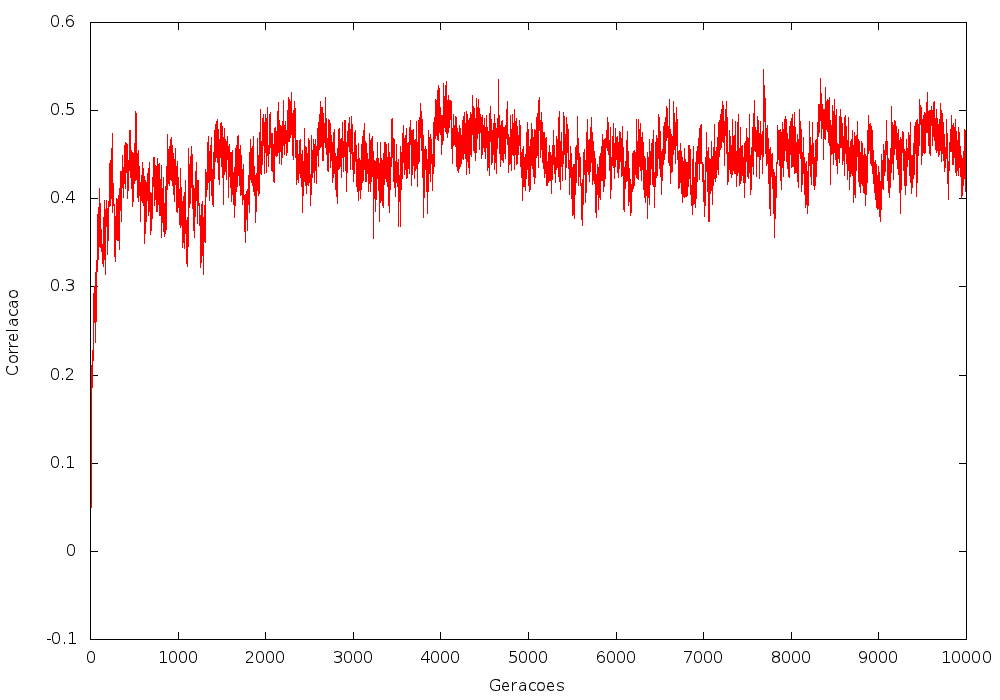
\includegraphics[width=150mm, height=80mm]{figuras/jones2tracos.png}
  \caption{Evolução da correlação entre dois caracteres ligados por efeitos
  mutacionais pleiotrópicos sobre seleção estabilizadora correlacionada.
  Nesta simulação $r_\omega=0.8$, $Ne=5.000$, $p=2$, $m=50$}
  \label{jones2tracos}
\end{figure}


Como nosso objetivo é expandir a modelagem para mais caracteres, em seguida
adicionamos um caráter ao sistema. 
Nesse caso, as considerações sobre a dificuldade de manter a matriz $M$
positiva definida já se aplicam, sendo necessário fazer uso da correção
de autovalores. 
Mesmo assim, o resultado é bastante semelhante, ainda com a correlação
entre os 3 caracteres se alinhando com a matriz $\omega$ (figuras
\ref{jones3tracos} e \ref{MatJones3tracos}). 


\begin{figure}[htbp]
  \centering
  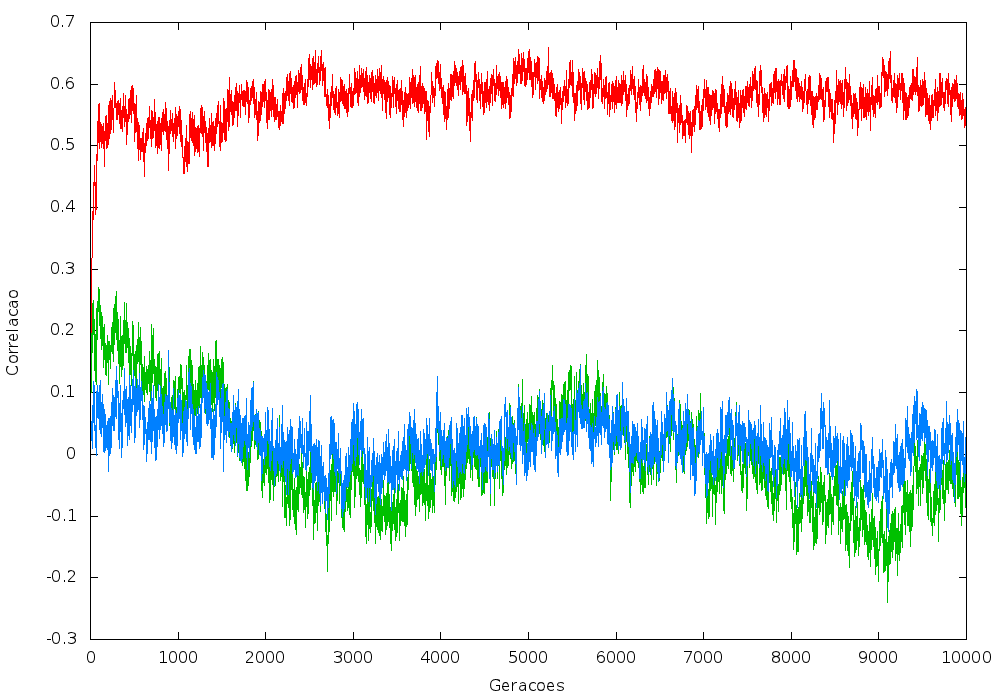
\includegraphics[width=150mm, height=80mm]{figuras/jones3tracos.png}
  \caption{Evolução da correlação entre três caracteres ligados por efeitos
  mutacionais pleiotrópicos sobre seleção estabilizadora correlacionada.
  A seleção propicia a integração entre dois caracteres (linha vermelha) e a desintegração
  desses dois com o terceiro (linhas azul e verde). Nesta simulação
  $r_\omega$ como na equação \ref{romega}, $Ne=5.000$, $p=3$, $m=50$.}
  \label{jones3tracos}
\end{figure}


Na figura \ref{MatJones3tracos} vemos representações gráficas da matriz
de correlação fenotípica ao final da simulação e da matriz $\omega$ de
seleção estabilizadora correlacionada. 
Caselas mais claras indicam correlação maior. 
Nesse caso, a matriz de correlação da superfície de seleção foi:

\begin{equation}
Corr(\omega) = \left( \begin{smallmatrix} 1 & 0.9 & 0.1\\  0.9 & 1 & 0.1 \\ 0.1 & 0.1 & 1 \end{smallmatrix}  \right)
\label{romega}
\end{equation}

E a matriz de covariância da superfície de seleção: 

\begin{equation}
\omega = \left( \begin{smallmatrix} 9 & 8.1 & 0.9\\  8.1 & 9 & 0.9 \\ 0.9 & 0.9 & 9 \end{smallmatrix}  \right)
\end{equation}


\begin{figure}[htbp]
  \centering
  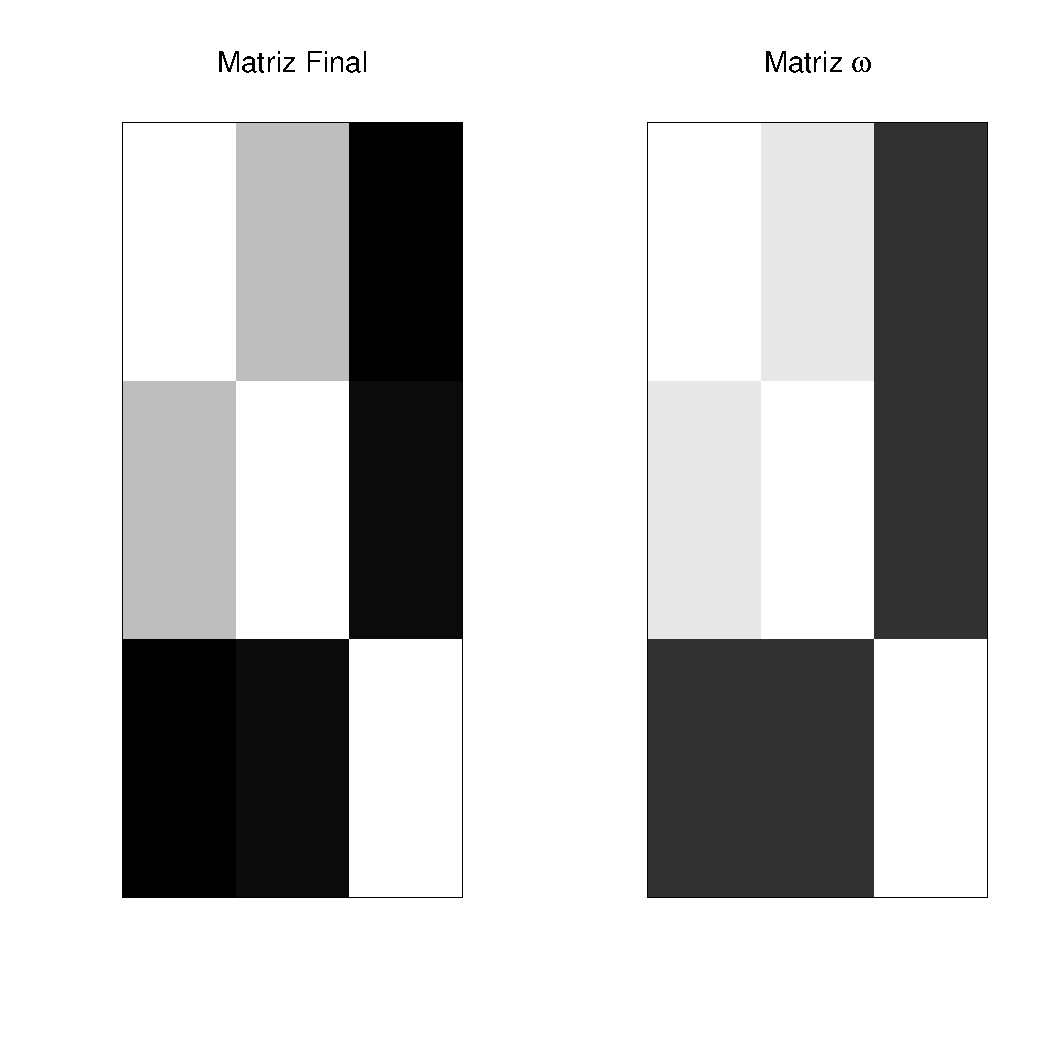
\includegraphics[width=150mm, height=80mm]{figuras/Mat3tracos}
   \caption{Comparação entre a matriz de correlação final para 3
   caracteres após 10.000
   gerações de seleção e a matriz $\omega$ da superfície de seleção.}
  \label{MatJones3tracos}
\end{figure}


Quando procuramos ampliar o número de caracteres, porém, o alinhamento da
matriz G com a matriz $\omega$ se mostrou problemático. 
Nesse caso a matriz de correlação da superfície de seleção continha dois
módulos, e era dada por:

\begin{equation}
Corr(\omega) = \left( 
\begin{smallmatrix} 
1 & 0.8 & 0.8 & 0.8 & 0.8 & 0 & 0 & 0 & 0 & 0\\  
0.8 & 1 & 0.8 & 0.8 & 0.8 & 0 & 0 & 0 & 0 & 0\\  
0.8 & 0.8 & 1 & 0.8 & 0.8 & 0 & 0 & 0 & 0 & 0\\  
0.8 & 0.8 & 0.8 & 1 & 0.8 & 0 & 0 & 0 & 0 & 0\\  
0.8 & 0.8 & 0.8 & 0.8 & 1 & 0 & 0 & 0 & 0 & 0\\  
0 & 0 & 0 & 0 & 0 & 1 & 0.8 & 0.8 & 0.8 & 0.8\\ 
0 & 0 & 0 & 0 & 0 & 0.8 & 1 & 0.8 & 0.8 & 0.8\\
0 & 0 & 0 & 0 & 0 & 0.8 & 0.8 & 1 & 0.8 & 0.8\\
0 & 0 & 0 & 0 & 0 & 0.8 & 0.8 & 0.8 & 1 & 0.8\\
0 & 0 & 0 & 0 & 0 & 0.8 & 0.8 & 0.8 & 0.8 & 1
\end{smallmatrix}  \right)
\label{matw}
\end{equation}

Na figura \ref{jones10tracos} vemos a trajetória típica das correlações
fenotípicas com uma matriz $\omega$ com dois módulos (ver figura
\ref{MatJones10tracos}).  
Aqui não existe mais a distinção entre
correlações dentro de módulos (altas) e entre módulos (baixas). 
Os resultados da evolução da modularidade $L$ e do AVG-Ratio confirmam a
ausência de modularização do sistema. 
A modularidade $L$ apresenta uma leve subida ao longo da simulação, mas
o AVG-Ratio permanece estável (Figura \ref{jones10tracosStats}). 
Isso se deve à modularidade $L$ capturar qualquer tipo de modularidade
na matriz, não só aquela associada a superfície de seleção. 
Na figura \ref{MatJones10tracos} fica claro que não existe semelhança
entre as matrizes G e $\omega$. 
Realizamos essas simulações com uma gama grande de intensidades de
seleção e chegando até 100.000 gerações de seleção, sem nenhum indício de
alinhamento entre as matrizes G e $\omega$.  


\begin{figure}[htbp]
  \centering
  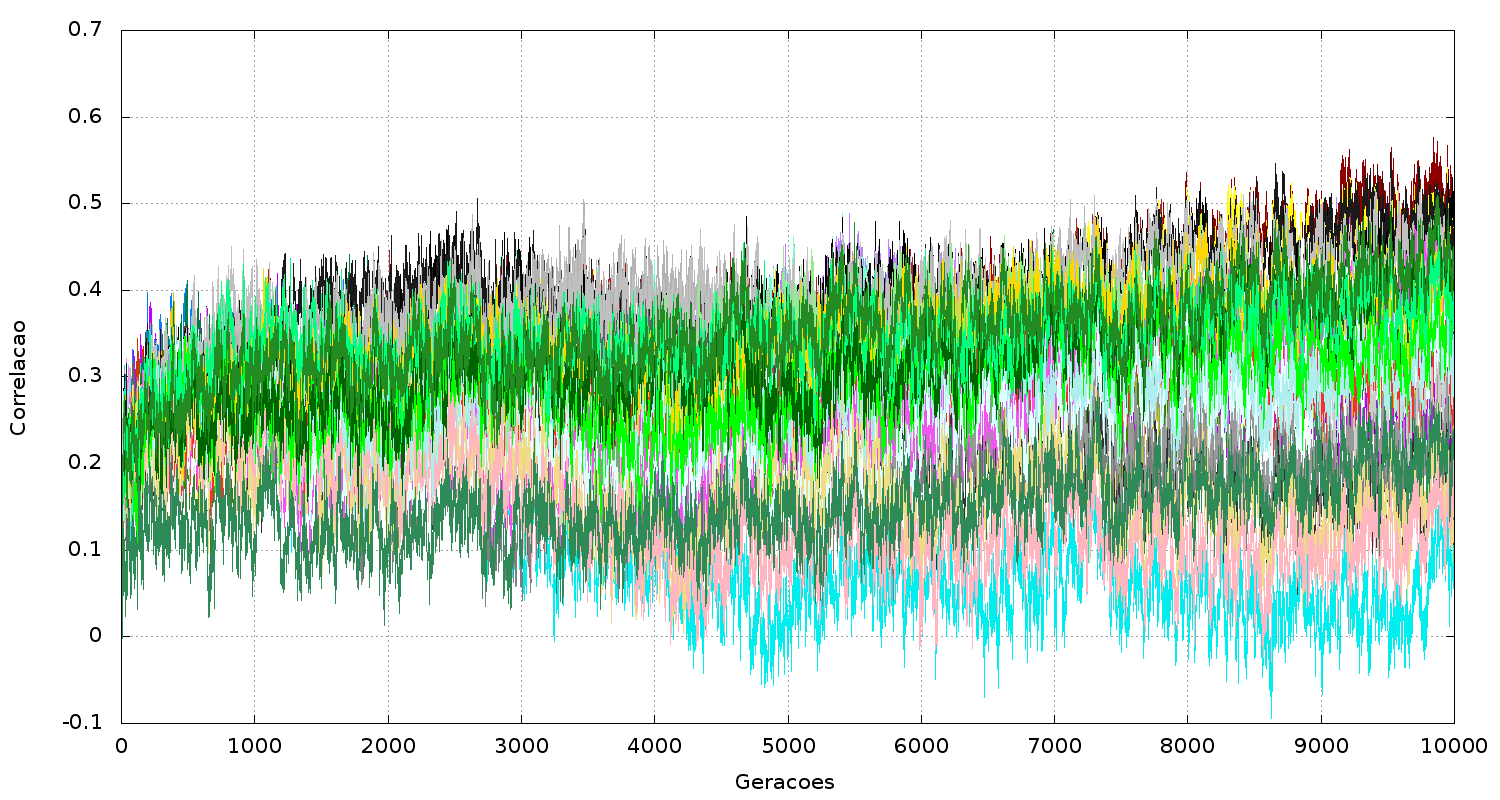
\includegraphics[width=150mm, height=80mm]{figuras/jones10tracos.png}
  \caption{Evolução da correlação entre dez caracteres ligados por efeitos
  mutacionais pleiotrópicos sobre seleção estabilizadora
  correlacionada. Apesar de a seleção promover a integração entre os
  5 primeiros e os 5 últimos caracteres e a desintegração entre esse
  módulos, isso não se transmite à matriz de correlação. Nesta simulação
  $r_\omega$ como na equação \ref{matw}, $Ne=5.000$, $p=10$, $m=50$.}
  \label{jones10tracos}
\end{figure}



\begin{figure}[htbp]
  \centering
  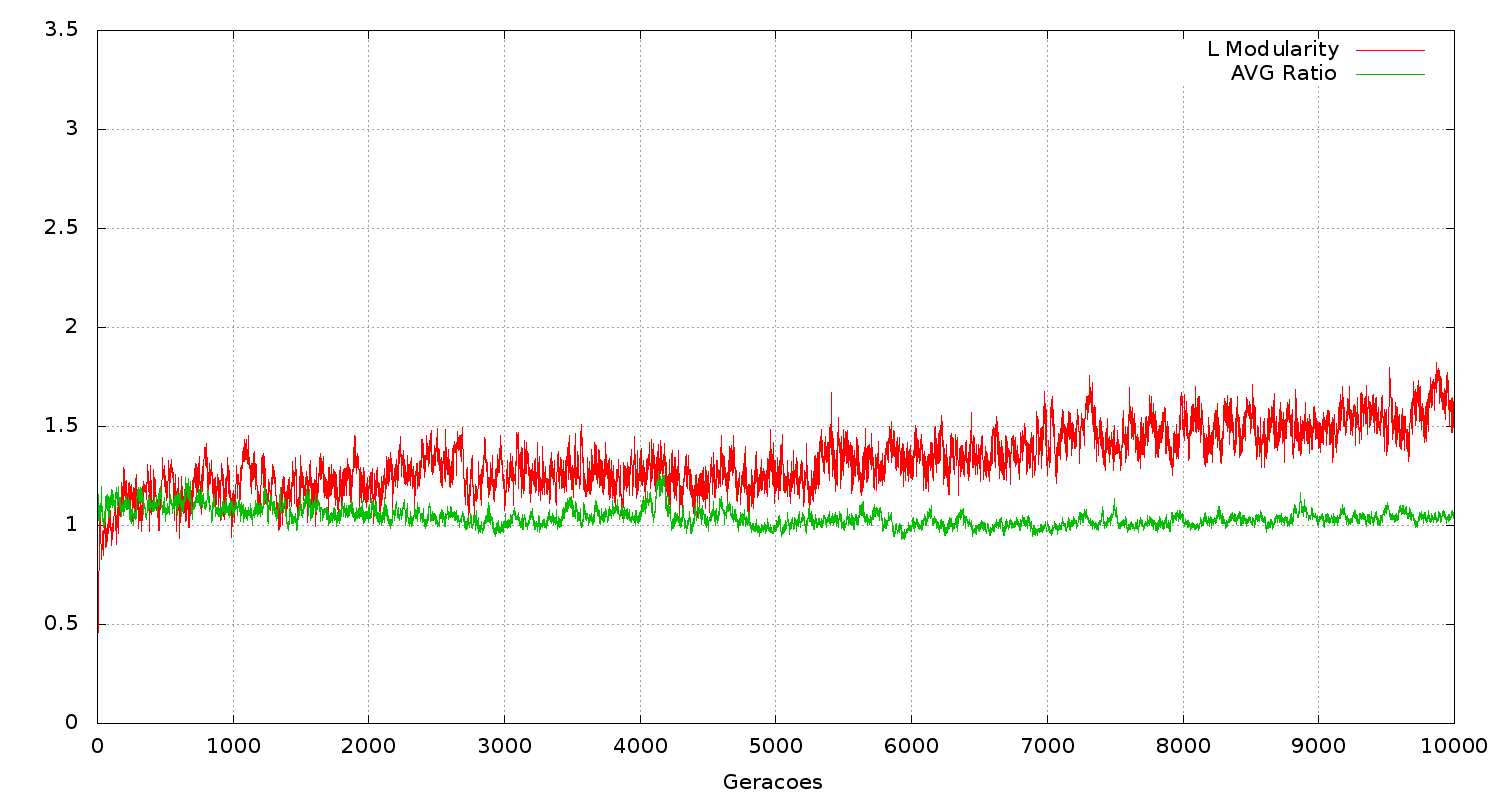
\includegraphics[width=150mm, height=80mm]{figuras/jones10tracosStats.png}
  \caption{Evolução da modularidade $L$ e AVG-Ratio para as matrizes de
  correlação representadas na figura \ref{jones10tracos}}
  \label{jones10tracosStats}
\end{figure}



\begin{figure}[htbp]
  \centering
  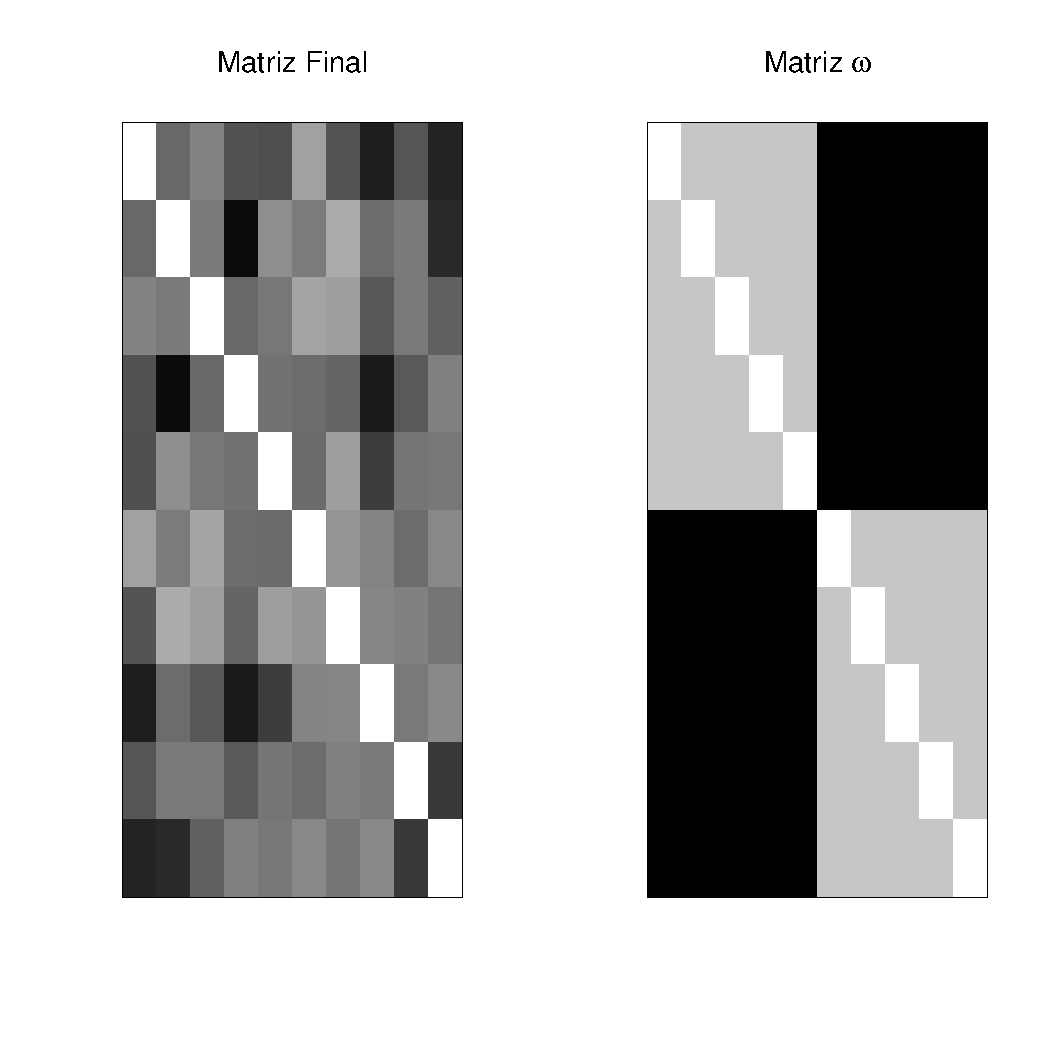
\includegraphics[width=150mm, height=80mm]{figuras/Mat10tracos}
  \caption{Comparação entre a matriz de correlação final para 10
  caracteres após 10.000 gerações de seleção representadas na figura
  \ref{jones10tracos} e a matriz $\omega$ da superfície de seleção.}
  \label{MatJones10tracos}
\end{figure}



\subsection{Seleção Direcional}

Em seguida, procuramos explorar como a inclusão de seleção direcional afetaria o
alinhamento das matrizes G e $\omega$. 
Utilizamos novamente uma matriz $\omega$ modular e acrescentamos seleção
direcional correlacionada, de mudança conjunta na média dos caracteres
dentro de cada um dos módulos, e mudanças antagônicas entre módulos. 
Ou seja, os 5 primeiros caracteres tiveram seu ótimo fenotípico aumentado a
uma taxa constante e os 5 últimos caracteres tiveram seu ótimo reduzido de
forma simétrica ($\Delta_S=0.2$). 
As populações respondem a essa seleção de forma eficiente, alterando
suas médias de acordo com a posição do ótimo. 
Após 10.000 gerações de seleção direcional, observamos a matriz final
e a evolução de todas as correlações genéticas nesse período. 
Os resultados podem ser vistos nas figuras \ref{jones10tracosDirecional}
, \ref{jones10tracosDirecionalStats} e \ref{MatJones10tracosDirecional}. 
Mesmo nessas condições, não observamos a emergência de módulos
variacionais na matriz G, que indicaria semelhança com a matriz $\omega$
e o padrão de seleção direcional correlacionada. 


\begin{figure}[htbp]
  \centering
  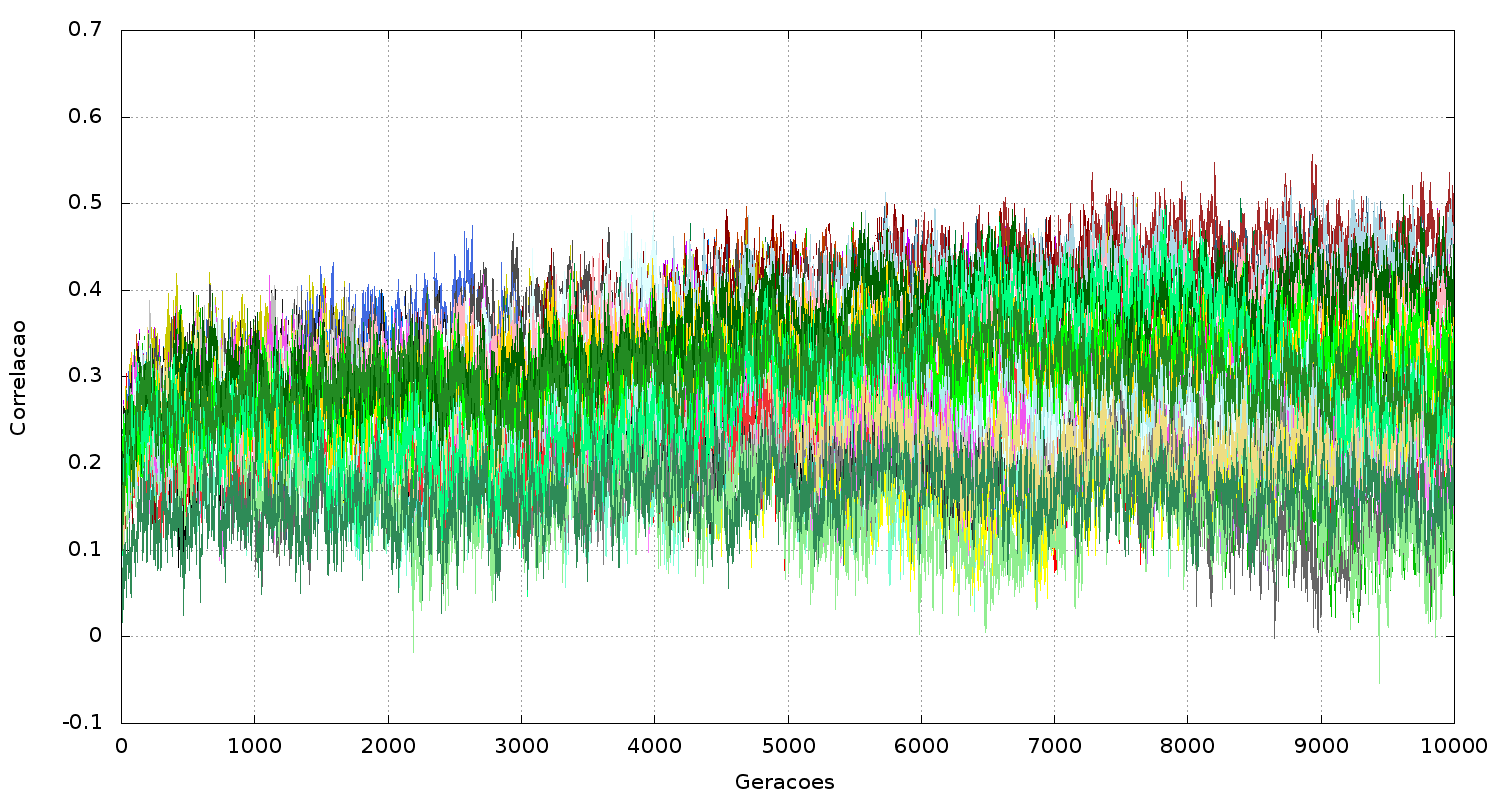
\includegraphics[width=150mm, height=80mm]{figuras/jones10tracosDirecional.png}
  \caption{Evolução da correlação entre dez caracteres ligados por efeitos
  mutacionais pleiotrópicos sobre seleção estabilizadora correlacionada
  e seleção direcional intensa para mudança correlacionada dentro dos
  módulos. Novamente, isso não se traduz na matriz de correlação genética.}
  \label{jones10tracosDirecional}
\end{figure}



\begin{figure}[htbp]
  \centering
  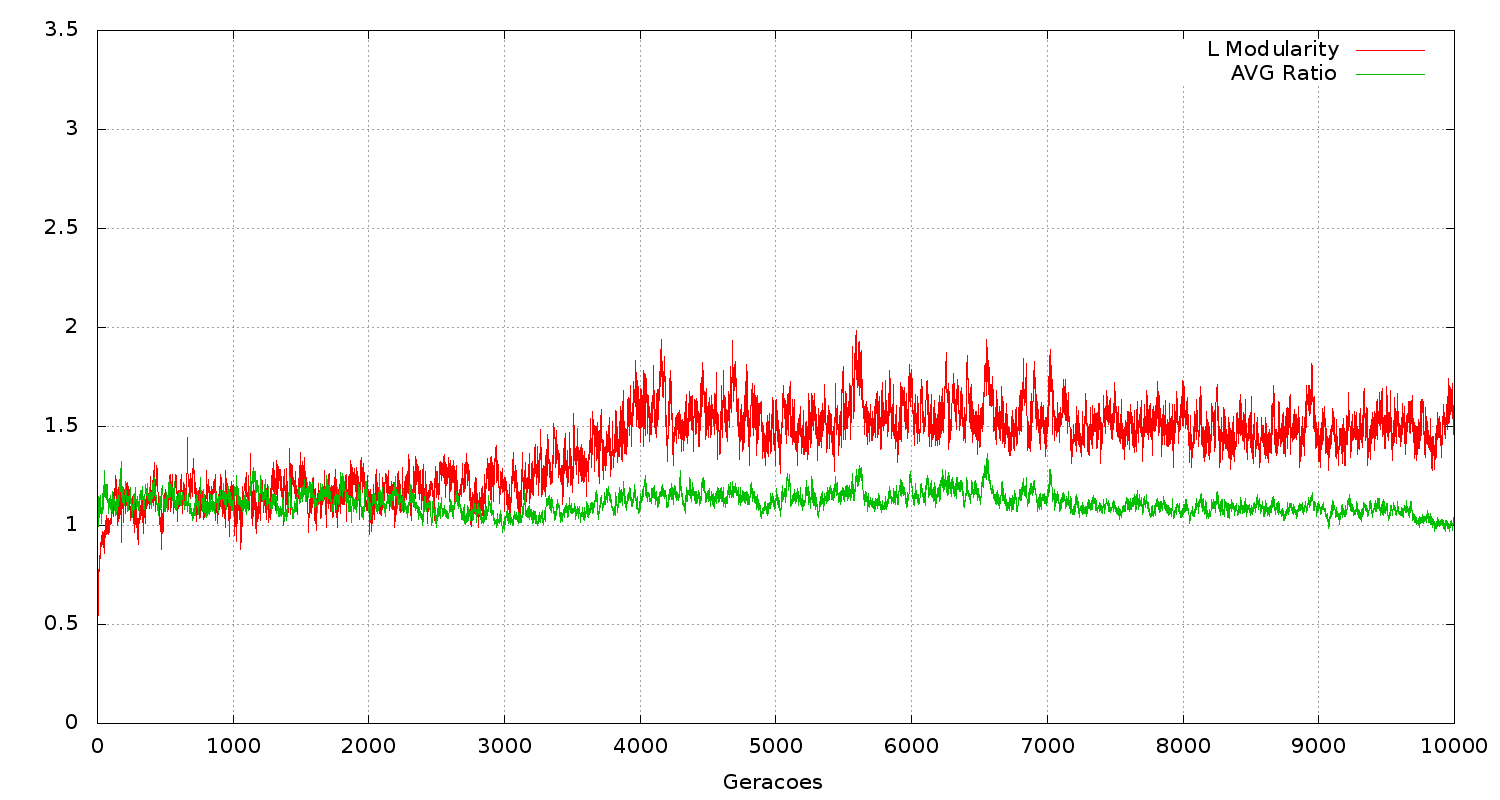
\includegraphics[width=150mm, height=80mm]{figuras/jones10tracosDirecionalStats.png}
  \caption{Evolução da modularidade $L$ e AVG-Ratio para as matrizes de
  correlação representadas na figura \ref{jones10tracosDirecional}}
  \label{jones10tracosDirecionalStats}
\end{figure}



\begin{figure}[htbp]
  \centering
  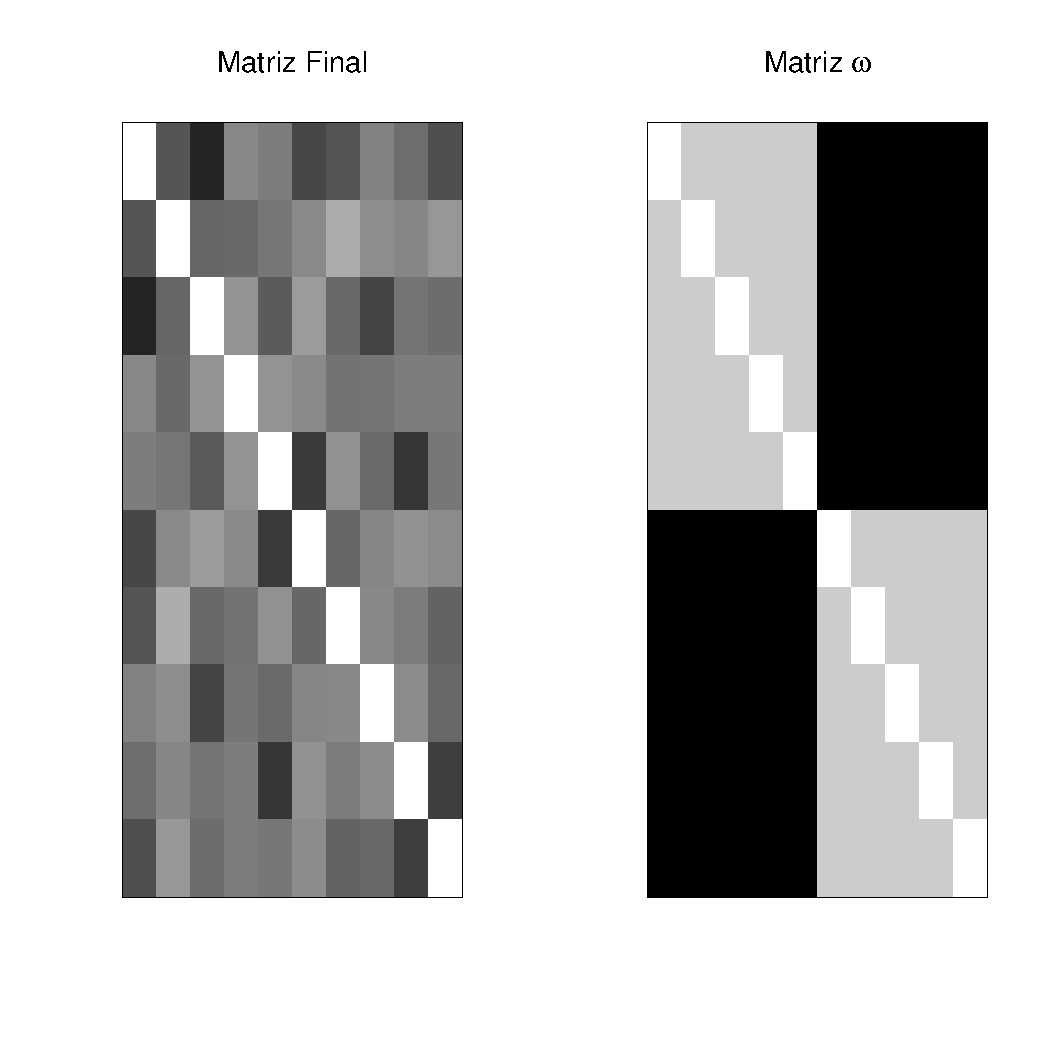
\includegraphics[width=150mm, height=80mm]{figuras/Mat10tracosDirecional}
   \caption{Comparação entre a matriz de correlação final para 10 caracteres
   após 10.000 gerações de seleção direcional e estabilizadora
   representadas na figura \ref{jones10tracosDirecional} com a matriz
   $\omega$ da superfície de seleção.}
  \label{MatJones10tracosDirecional}
\end{figure}


Acreditamos que essa dificuldade em reproduzir os resultados encontrados
em sistemas com 2 e 3 caracteres no sistema com 10 caracteres se deve ao aumento
considerável do espaço possível de variação que a inclusão de cada novo
caráter representa. 
O morfoespaço cresce rapidamente com a inclusão de cada novo caráter, e
o espaço permitido para a matriz $M$ também. 
A seleção indireta, então, se torna muito fraca para promover o
alinhamento entre as matrizes, e a mutação não explora de forma adequada
(ergódica) o espaço da matriz mutacional, levando a uma situação de não alinhamento
mesmo com uma pressão seletiva considerável. 
Claramente isso não é observado em sistemas naturais, onde populações
apresentam padrões modulares frequentemente associados a restrições
funcionais \citep{Porto2009}. 

\section{Resultados e Discussão $\cdot$ Matriz $B$}

Todas as simulações dessa seção começam com o mesmo estado inicial, com
a matriz $B$ totalmente formada por $1$, ou seja, integração total, e
todos os valores aditivos $0$, ou seja, todos os caracteres nulos. 
As primeiras gerações são dependentes desses estado inicial e não trazem
informação. 
Após cerca de $2.000$ gerações o sistema se encontra em equilíbrio
seleção-mutação-deriva e pode ser analisado independentemente do estado
inicial. 
Isso se reflete em todos os gráficos como um transiente instável, seguido
de estabilidade dependente principalmente do tamanho populacional.
Discutimos esses efeitos e outros na próxima seção. 

\subsection{Seleção Estabilizadora}

No segundo tipo de modelagem, começamos já com 10 caracteres sofrendo
seleção estabilizadora correlacionada dada pela matriz apresentada na
equação \ref{matw}. 
Exploramos então a influência de várias razões entre a taxa de mutação
nos alelos aditivos ($\mu$) e a taxa de mutação nas caselas da matriz
$B$ ($\mu_B$). 
Essa razão $\mu/\mu_B$ define como será a dinâmica temporal de mudança
entre dois níveis: o dos efeitos aditivos e o da atribuição desses
efeitos aos caracteres quantitativos, que chamamos aqui de efeito {\it ontogenético}. 
Conforme vemos nas figuras \ref{MatBEstab} e \ref{EstabRMuStats}, apesar de mudanças na
magnitude das correlações com o aumento da razão $\mu/\mu_B$, não
observamos o surgimento de módulos variacionais apenas com seleção
estabilizadora correlacionada. 


\begin{figure}[htbp]
  \centering
  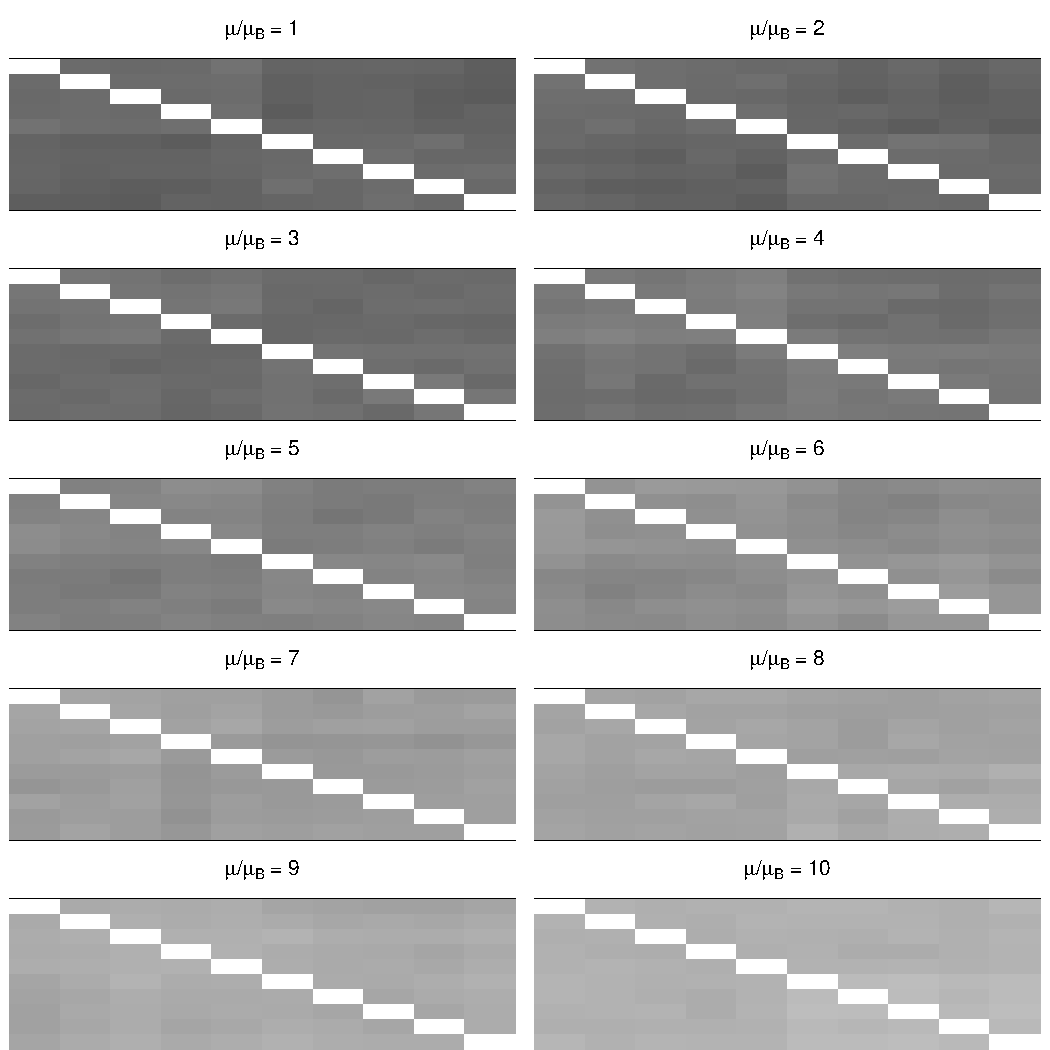
\includegraphics[width=150mm, height=180mm]{figuras/MatBEstabRMu}
   \caption{Matriz final média de 10 corridas para diferentes razões de
   $\mu$ e $\mu_B$, com seleção estabilizadora correlacionada com 2
   módulos.}
  \label{MatBEstab}
\end{figure}



\begin{figure}[htbp]
   \centering
   \subfloat [$\mu/\mu_B = 1$]{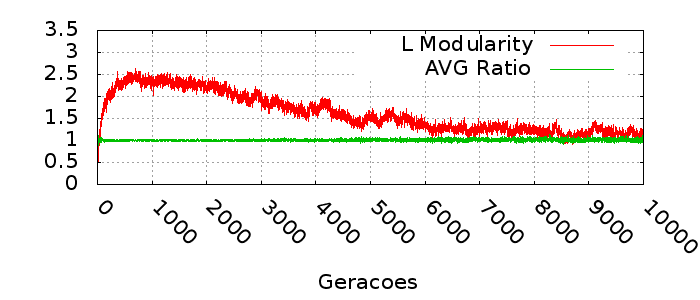
\includegraphics[width=70mm, height=30mm]{figuras/EstabRMuStats1.png}}\vspace{11pt}
   \subfloat [$\mu/\mu_B = 2$]{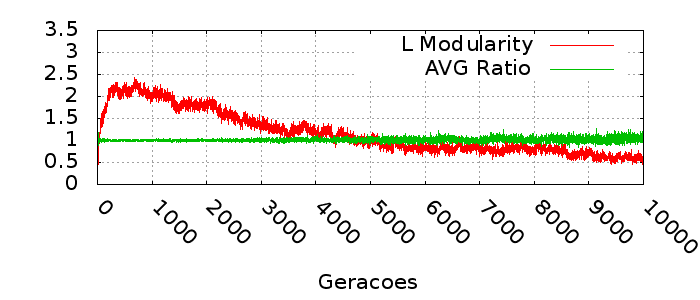
\includegraphics[width=70mm, height=30mm]{figuras/EstabRMuStats2.png}}\\ 
   \vspace{-18pt}
   \subfloat [$\mu/\mu_B = 3$]{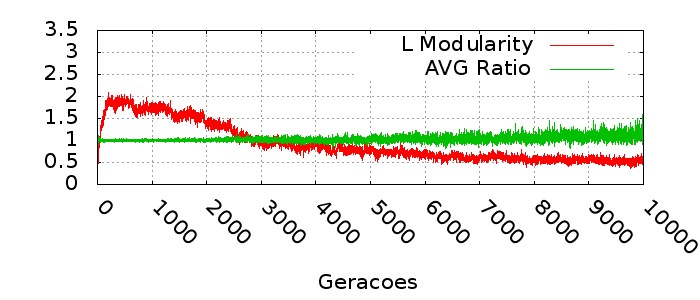
\includegraphics[width=70mm, height=30mm]{figuras/EstabRMuStats3.png}}\vspace{11pt} 
   \subfloat [$\mu/\mu_B = 4$]{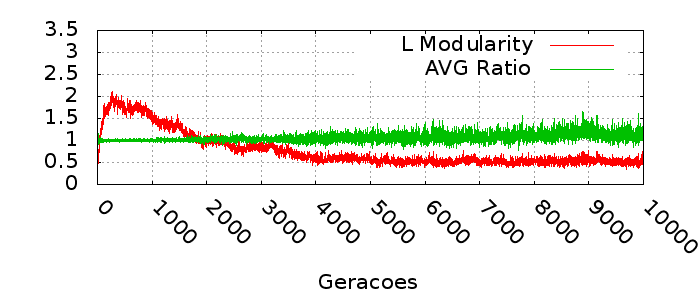
\includegraphics[width=70mm, height=30mm]{figuras/EstabRMuStats4.png}}\\
   \vspace{-18pt}
   \subfloat [$\mu/\mu_B = 5$]{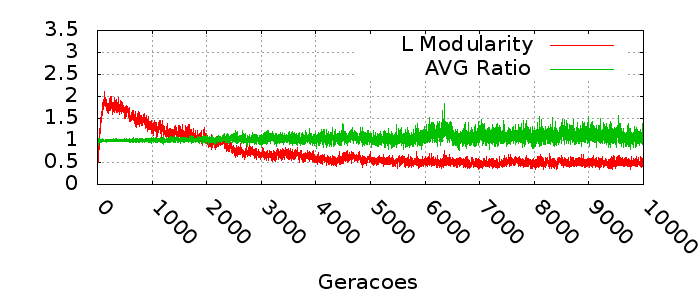
\includegraphics[width=70mm, height=30mm]{figuras/EstabRMuStats5.png}}\vspace{11pt}
   \subfloat [$\mu/\mu_B = 6$]{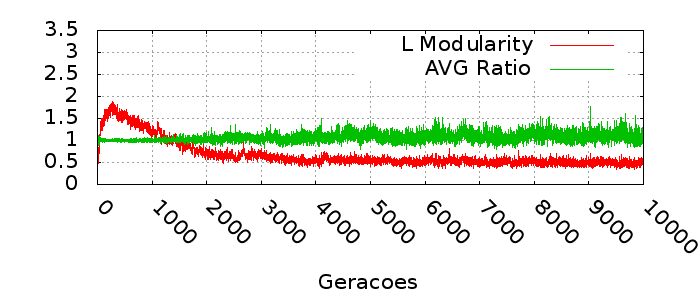
\includegraphics[width=70mm, height=30mm]{figuras/EstabRMuStats6.png}}\\
   \vspace{-18pt}
   \subfloat [$\mu/\mu_B = 7$]{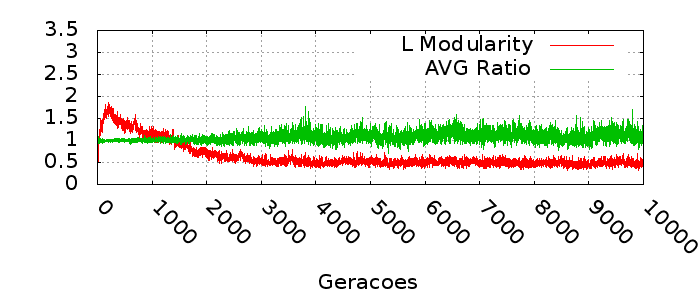
\includegraphics[width=70mm, height=30mm]{figuras/EstabRMuStats7.png}}\vspace{11pt}
   \subfloat [$\mu/\mu_B = 8$]{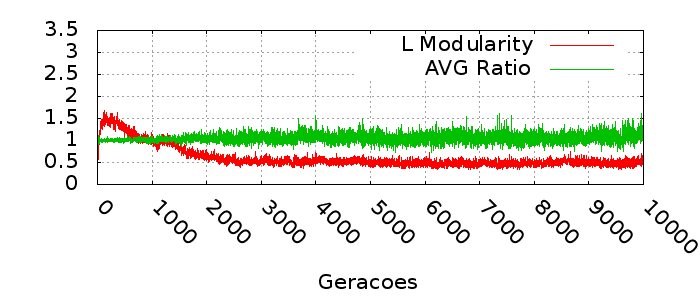
\includegraphics[width=70mm, height=30mm]{figuras/EstabRMuStats8.png}}\\
   \vspace{-18pt}
   \subfloat [$\mu/\mu_B = 9$]{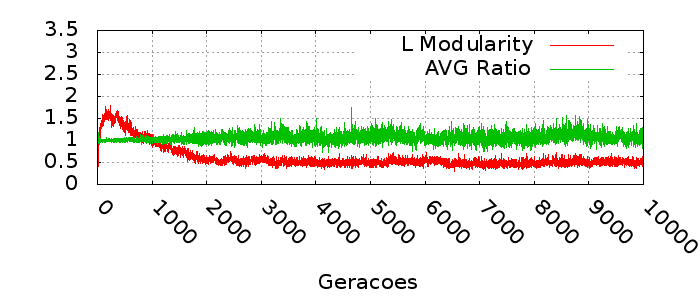
\includegraphics[width=70mm, height=30mm]{figuras/EstabRMuStats9.png}}\vspace{11pt}
   \subfloat [$\mu/\mu_B = 10$]{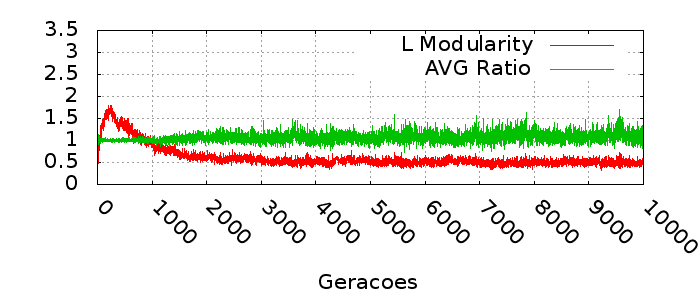
\includegraphics[width=70mm, height=30mm]{figuras/EstabRMuStats10.png}}\\
   \caption{Evolução típica de AVG-Ratio e modularidade $L$ para diferentes razões de
   $\mu$ e $\mu_B$, com seleção estabilizadora correlacionada com 2 módulos.}
   \label{EstabRMuStats}
\end{figure}



\subsection{Seleção Direcional}
\label{cap3:DirecB}

Com a inclusão de seleção direcional, como na figura
\ref{MatJones10tracosDirecional}, e $\mu/\mu_B = 0.1$, ainda não
observamos a formação de módulos na matriz G (figura \ref{RMu01}). 
Porém, como vemos na figura \ref{MatBDirecional-RMu}, o aumento  na
razão $\mu/\mu_B$ aliada à seleção direcional é capaz de alterar esse
comportamento. 
Esse aumento parece promover um sistema capaz de responder de forma
eficiente às pressões seletivas impostas e gerar uma matriz G com a
estrutura modular privilegiada pela seleção estabilizadora e direcional. 
Lembramos que na ausência de seleção direcional esse efeito não é
observado, mesmo com as mesmas razões $\mu/\mu_B$. 
Na figura \ref{DirecionalRMuStats} vemos que razões baixas de $\mu/\mu_B$ levam
a sistemas bastante instáveis, apesar de modulares. 
Novamente isso pode ser interpretado como uma consequência de taxas de
mudança em cada nível da simulação incompatíveis com populações
estáveis. 
Para $\mu/\mu_B=1$, ou seja, com a taxa de mutação igual nos níveis
aditivo e ontogenético, o valor de modularidade $L$ flutua violentamente entre
as gerações, sugerindo uma modularidade muito instável. 
As mudanças ``regulatórias'' da matriz $B$ não podem se dar na mesma
escala temporal das mudanças aditivas, ou o sistema não tem tempo de
responder a seleção de forma estável. 
A partir de $\mu/\mu_B=4$ o sistema se torna muito mais estável e
progressivamente menos modular. 
Nós optamos por utilizar o valor $\mu/\mu_B=5$ nas simulações
subsequentes. 
Essa opção se deu por uma série de fatores: nesse valor o sistema ainda
apresenta um aumento de modularidade ao longo das gerações; os valores
de modularidade $L$ e AVG-Ratio são bastante concordantes, sugerindo que
os módulos favorecidos pela seleção estão efetivamente sendo expressos
na população; e, por último, o sistema possui uma estabilidade razoável
sem se tornar incapaz de responder a seleção. 


\begin{figure}[htbp]
   \centering
   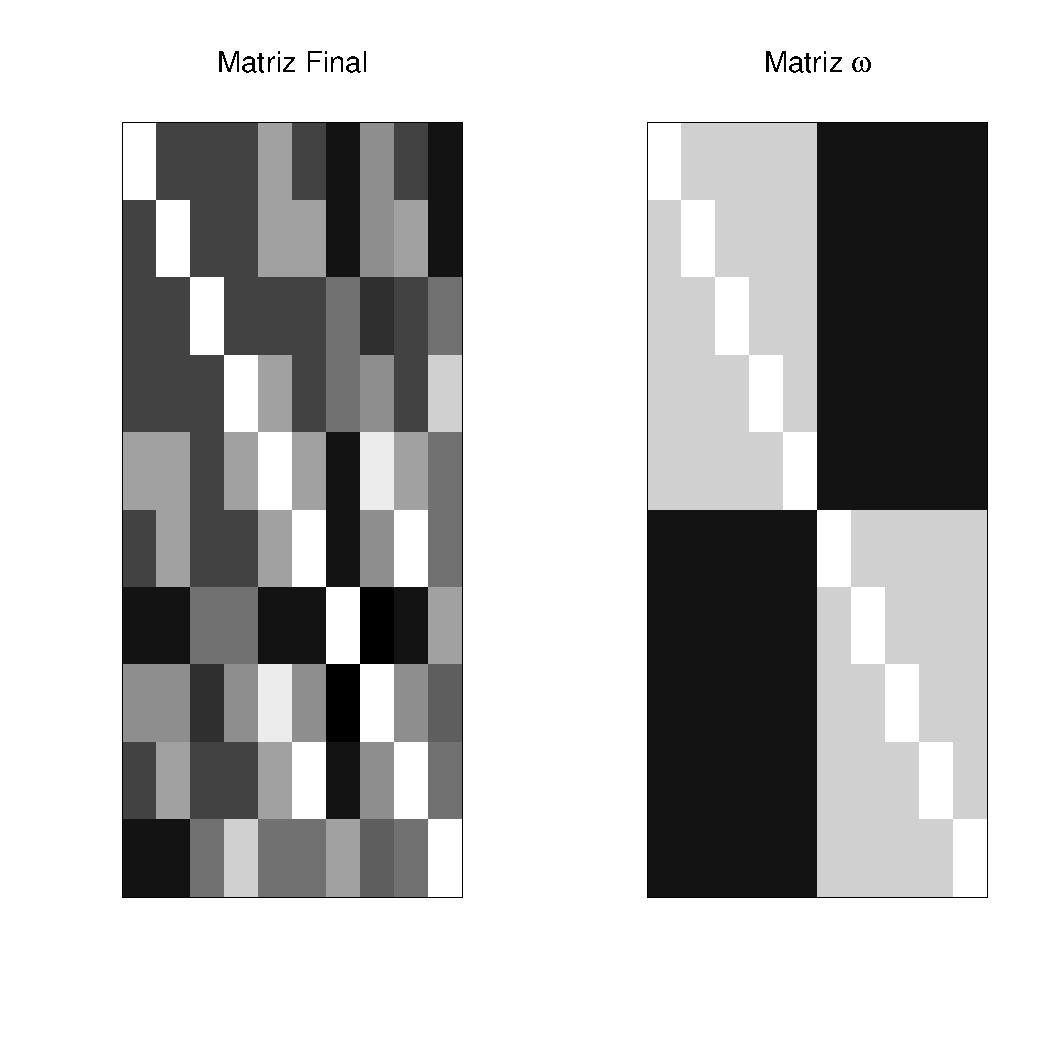
\includegraphics[width=150mm, height=80mm]{figuras/RMu01Omega}
   \caption{Comparação entre a matriz de correlação final média de 10
      corridas para o 10 caracteres após 10.000 gerações de seleção direcional e
      estabilizadora com a matriz $\omega$ da superfície de seleção e
   $\frac{\mu}{\mu_B}=0.1$, $Ne=2.500$, $\Delta_S=0.2$, $m/p=2$}
   \label{RMu01}
\end{figure}


Na figura \ref{MatBDirecionalNe2500RMu5} vemos um exemplo de corrida com
$N_e = 2.500$ e $\mu/\mu_B=5$, mostrando claramente a separação de grupos
de correlação dentro de e entre módulos. 
Posteriormente, vamos explorar a influência do tamanho populacional na
estabilidade das matrizes geradas pelas nossas simulações (figura
\ref{posselecao}). 


\begin{figure}[htbp]
  \centering
  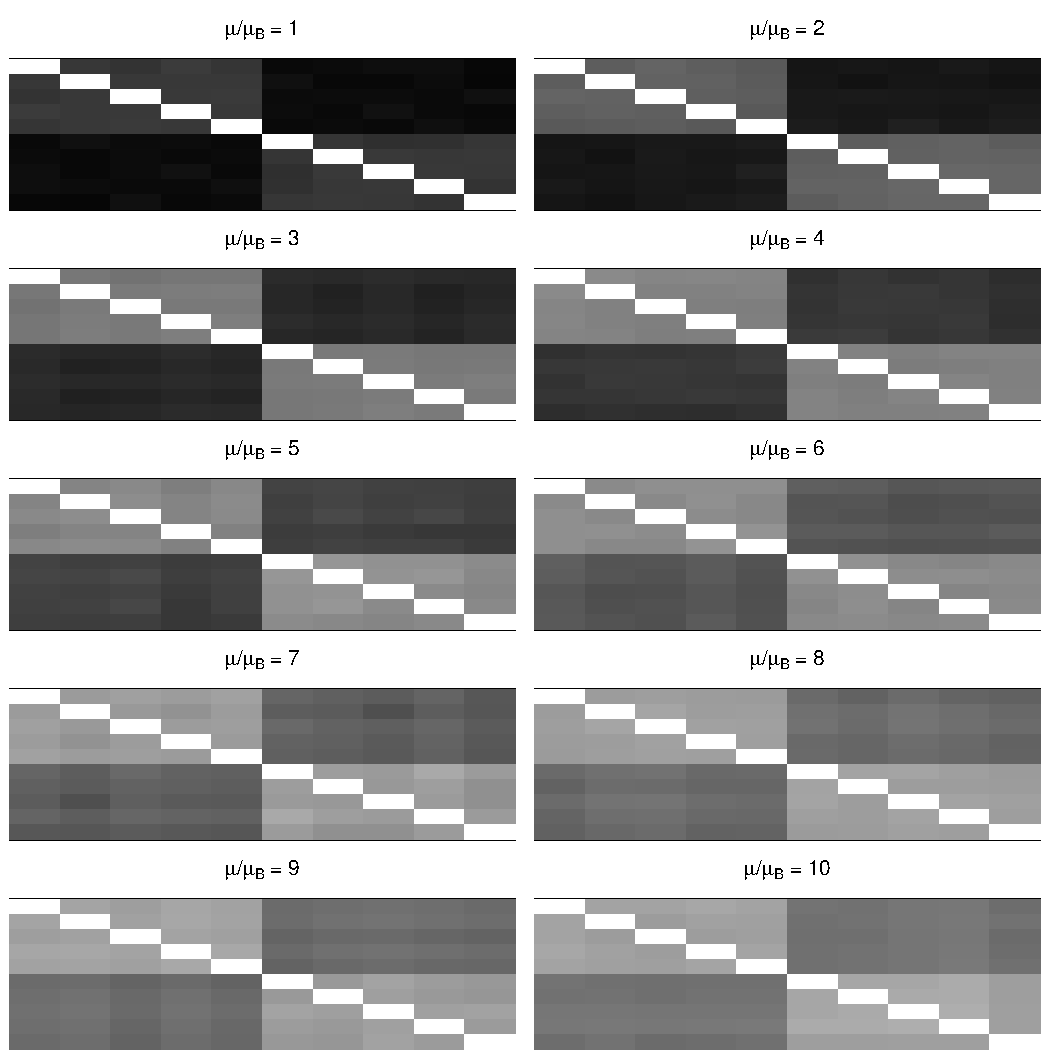
\includegraphics[width=150mm, height=180mm]{figuras/MatBDirecRMu}
   \caption{Matriz final média de 10 corridas para diferentes razões de
   $\frac{\mu}{\mu_B}$, com seleção estabilizadora correlacionada com 2
   módulos e seleção direcional correlacionada favorecendo os mesmos
   módulos. ($N_e=2.500$, $\Delta_S=0.2$, $m/n=2$)}
  \label{MatBDirecional-RMu}
\end{figure}



   \begin{figure}[htbp]
      \centering
      \subfloat [$\mu/\mu_B = 1$]{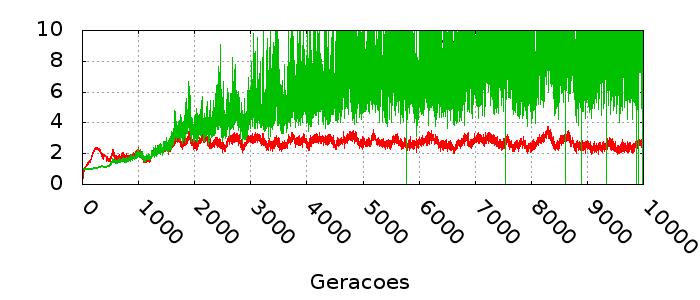
\includegraphics[width=70mm, height=30mm]{figuras/DirecionalRMuStats1.png}}\vspace{11pt}
      \subfloat [$\mu/\mu_B = 2$]{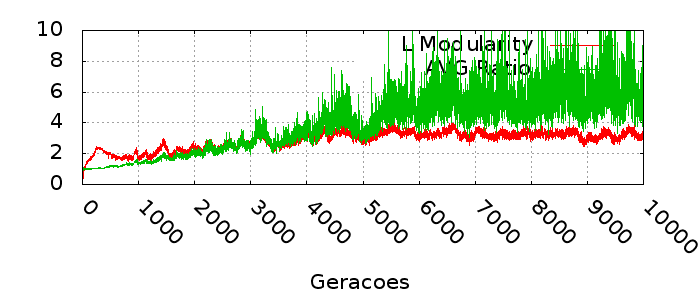
\includegraphics[width=70mm, height=30mm]{figuras/DirecionalRMuStats2.png}}\\ 
      \vspace{-18pt}
      \subfloat [$\mu/\mu_B = 3$]{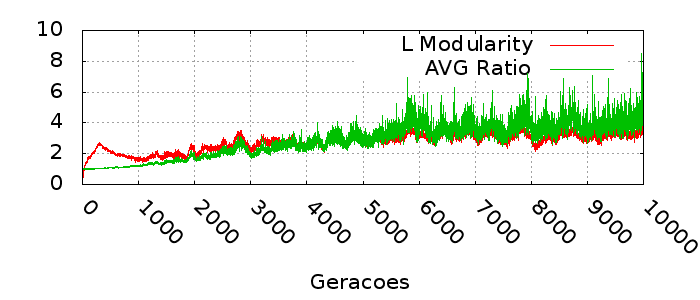
\includegraphics[width=70mm, height=30mm]{figuras/DirecionalRMuStats3.png}}\vspace{11pt} 
      \subfloat [$\mu/\mu_B = 4$]{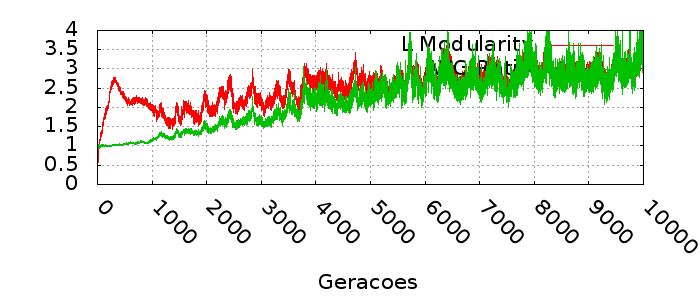
\includegraphics[width=70mm, height=30mm]{figuras/DirecionalRMuStats4.png}}\\
      \vspace{-18pt}
      \subfloat [$\mu/\mu_B = 5$]{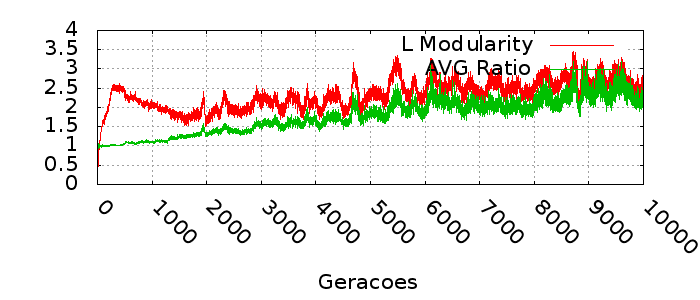
\includegraphics[width=70mm, height=30mm]{figuras/DirecionalRMuStats5.png}}\vspace{11pt}
      \subfloat [$\mu/\mu_B = 6$]{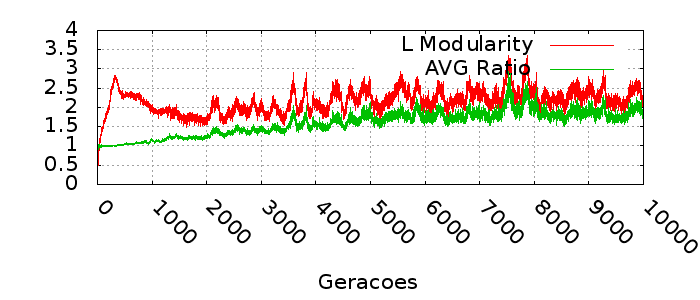
\includegraphics[width=70mm, height=30mm]{figuras/DirecionalRMuStats6.png}}\\
      \vspace{-18pt}
      \subfloat [$\mu/\mu_B = 7$]{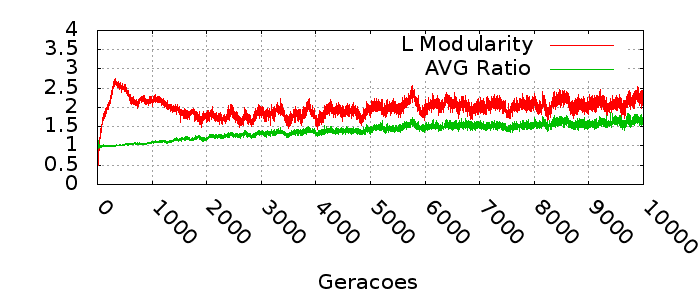
\includegraphics[width=70mm, height=30mm]{figuras/DirecionalRMuStats7.png}}\vspace{11pt}
      \subfloat [$\mu/\mu_B = 8$]{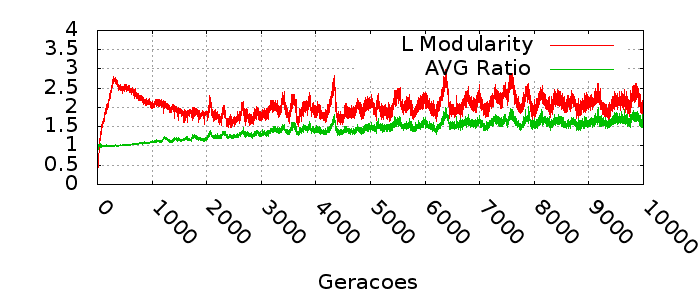
\includegraphics[width=70mm, height=30mm]{figuras/DirecionalRMuStats8.png}}\\
      \vspace{-18pt}
      \subfloat [$\mu/\mu_B = 9$]{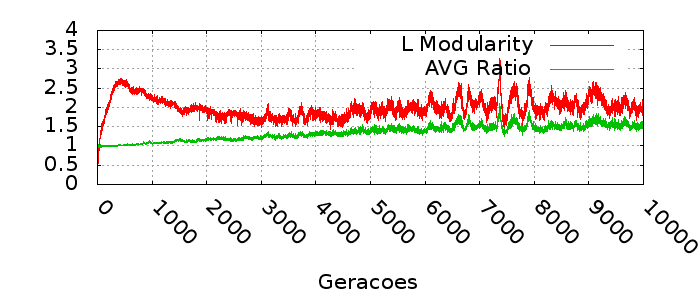
\includegraphics[width=70mm, height=30mm]{figuras/DirecionalRMuStats9.png}}\vspace{11pt}
      \subfloat [$\mu/\mu_B = 10$]{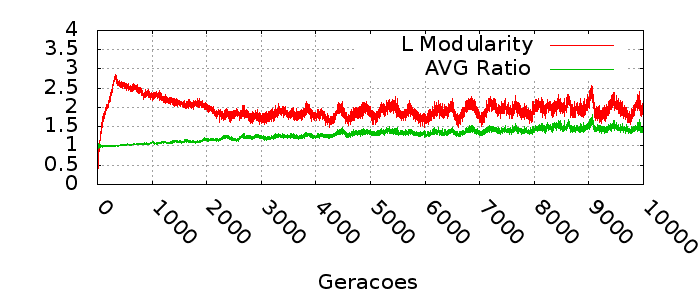
\includegraphics[width=70mm, height=30mm]{figuras/DirecionalRMuStats10.png}}\\
      \caption{Evolução típica de AVG-Ratio e modularidade $L$ para diferentes razões 
      $\mu/\mu_B$, com seleção estabilizadora correlacionada com 2
      módulos e seleção direcional correlacionada favorecendo os mesmos
      módulos. Atenção para a mudança de escala nos eixos verticais. ($N_e=2.500$, $\Delta_S=0.2$, $m/n=2$)}
      \label{DirecionalRMuStats}
   \end{figure}



\begin{figure}[htbp]
  \centering
  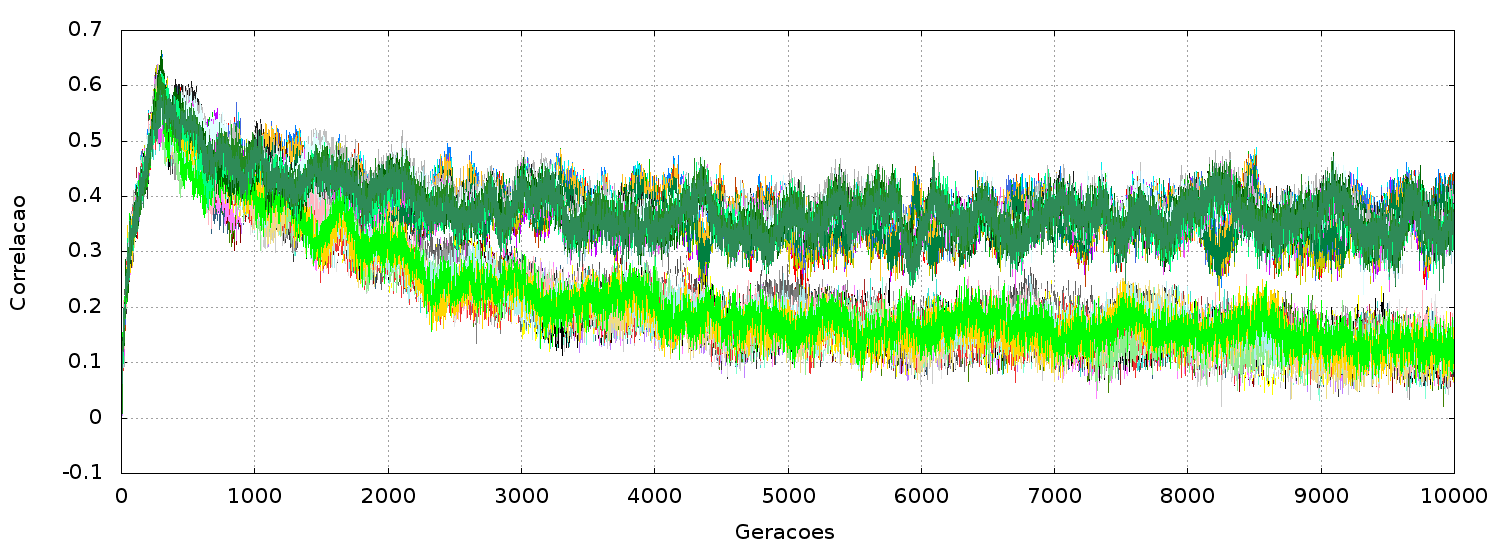
\includegraphics[width=150mm, height=55mm]{figuras/direcionalRMu5Ne2500IntSel200.png}
  \caption{Evolução da correlação entre dez caracteres ligados por efeitos
  pleiotrópicos controlados por uma função ontogenética linear binária
  variável, sofrendo seleção estabilizadora correlacionada
  e seleção direcional intensa para mudança correlacionada dentro dos
  módulos durante as 10.000 gerações. 
  ($N_e = 2.500$, $\mu/\mu_B=5$, $\Delta_S=0.2$, $m/p=2$)}
  \label{MatBDirecionalNe2500RMu5}
\end{figure}


Estamos interessados também na força de seleção direcional necessária
para gerar a estrutura modular nas matrizes de covariação. 
Nas figuras \ref{MatBIntSel110} e \ref{MatBIntSel1120} vemos matrizes
médias finais para 10 corridas com $N_e = 1.000$, $\mu/\mu_B=5$ e
intensidade de seleção variável. 
Para isso, modificamos o quanto o pico adaptativo era alterado para cada
caráter a cada geração, de $0.01$ até $0.2$ por geração durante 10.000
gerações. 
Nas figuras \ref{IntSelStats10100} e \ref{IntSelStats110200} vemos
evoluções típicas de AVG-Ratio e modularidade $L$ para corridas com
várias intensidades de seleção, mostrando o quão estáveis e o quão
rápido os padrões modulares se estabelecem nessas condições.
Vemos que mesmo com um tamanho populacional considerável ($Ne = 2.500$)
ainda observamos flutuações grandes. 

Quando aumentamos a intensidade de seleção, os módulos se tornam
mais evidentes, mas acima de uma certa intensidade (delta $\simeq 0.06$)
esse efeito se torna mais discreto. 
Esse platô na resposta a seleção direcional pode ser explicado por como
funciona a nossa seleção. 
Quando a variância entre as aptidões na população for suficientemente
alta, apenas os indivíduos com maior aptidão vão se reproduzir, e,
dentro de limites\footnote{ Quando o pico se encontra suficientemente
longe da média da população, a variância nos valores de aptidão cai
novamente, pois todos os indivíduos tem aptidão próxima de zero, e a
chance de um indivíduo se reproduzir deixa de depender do fenótipo. 
Isso é uma limitação do esquema de seleção estritamente gaussiano.}, as
mudanças em $\Delta_S$ não alteram quais são esses indivíduos. 


\begin{figure}[htbp]
  \centering
  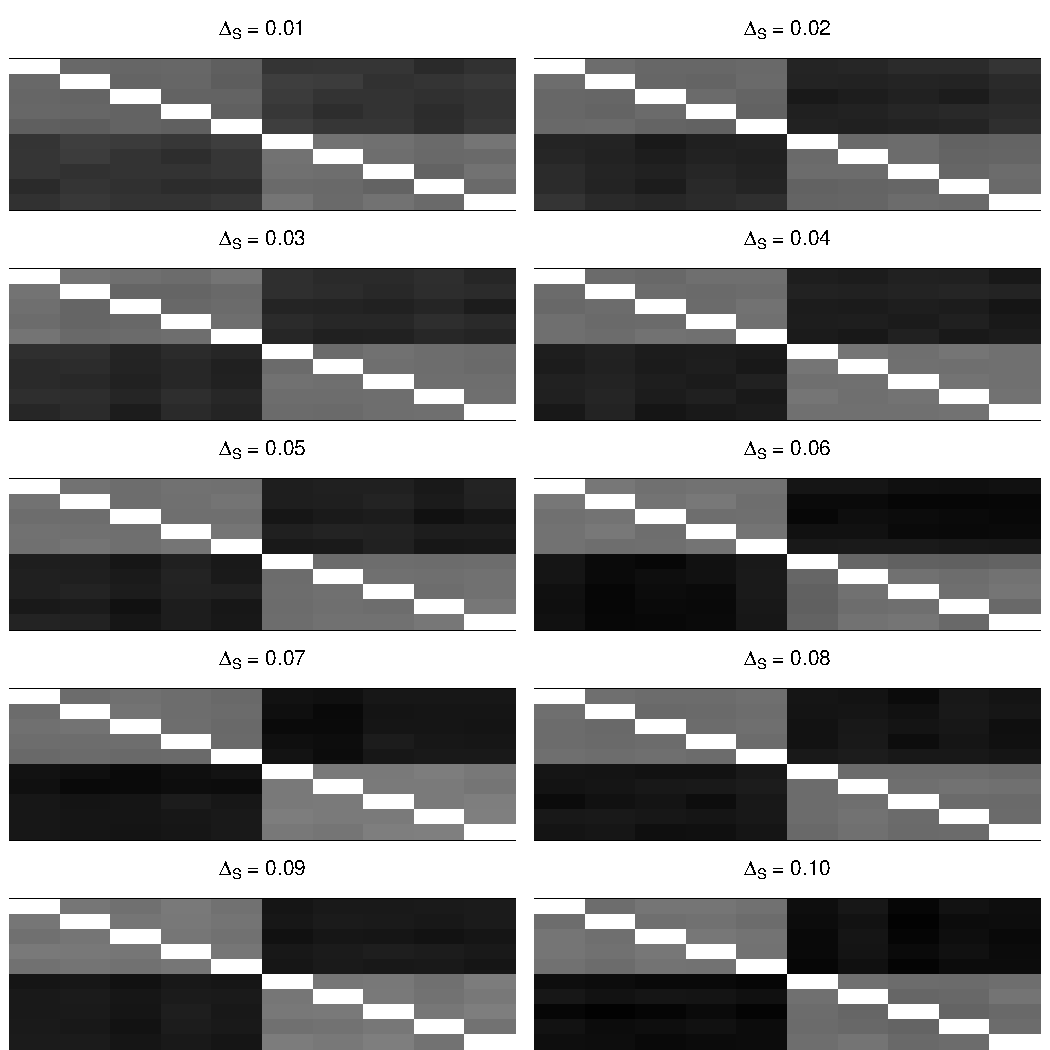
\includegraphics[width=150mm, height=180mm]{figuras/MatBDirecionalIntSel110}
   \caption{Matriz final média de 10 corridas com
   $\mu/\mu_B = 5$, $Ne = 1.000$, $m/p=2$, sofrendo seleção estabilizadora correlacionada com 2
   módulos e seleção direcional com diferentes valores de $\Delta_S$.}
  \label{MatBIntSel110}
\end{figure}



   \begin{figure}[htbp]
      \centering
      \subfloat [$\Delta_S = 0.01$]{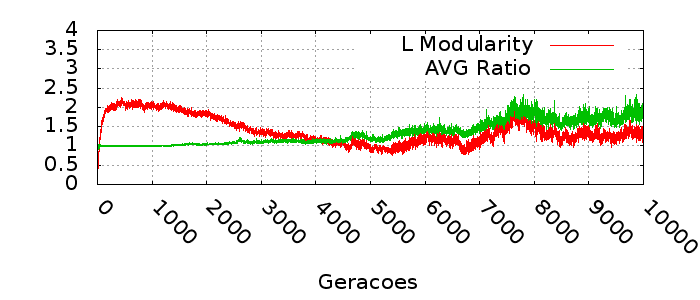
\includegraphics[width=70mm, height=30mm]{figuras/IntSelStats10.png}}\vspace{11pt}
      \subfloat [$\Delta_S = 0.02$]{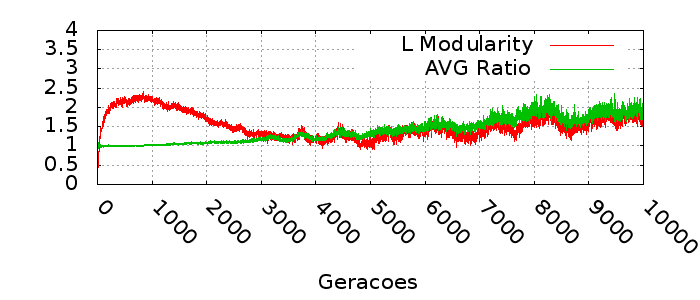
\includegraphics[width=70mm, height=30mm]{figuras/IntSelStats20.png}}\\ 
      \vspace{-18pt}
      \subfloat [$\Delta_S = 0.03$]{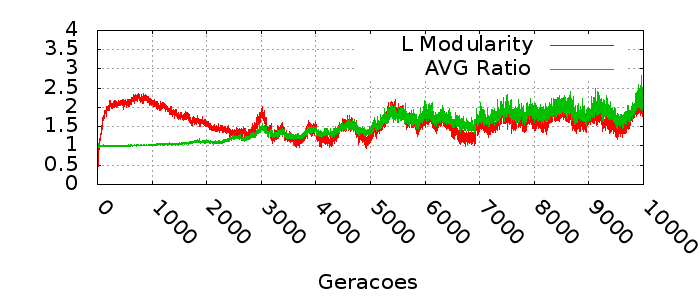
\includegraphics[width=70mm, height=30mm]{figuras/IntSelStats30.png}}\vspace{11pt} 
      \subfloat [$\Delta_S = 0.04$]{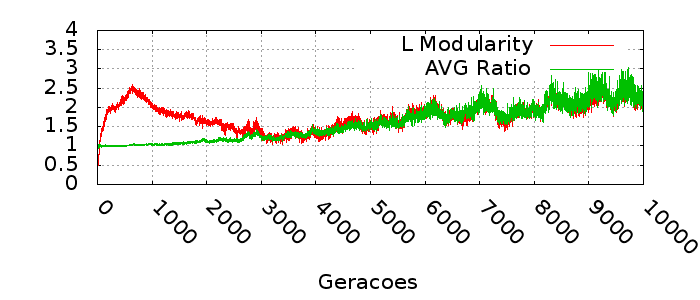
\includegraphics[width=70mm, height=30mm]{figuras/IntSelStats40.png}}\\
      \vspace{-18pt}
      \subfloat [$\Delta_S = 0.05$]{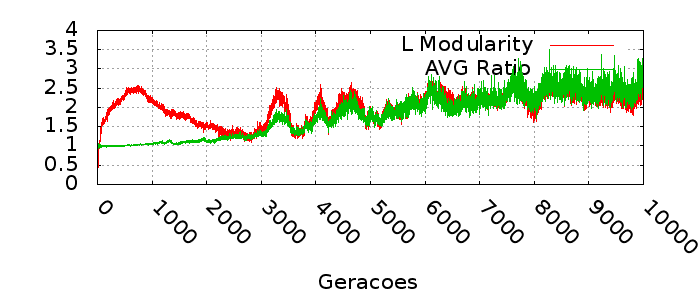
\includegraphics[width=70mm, height=30mm]{figuras/IntSelStats50.png}}\vspace{11pt}
      \subfloat [$\Delta_S = 0.06$]{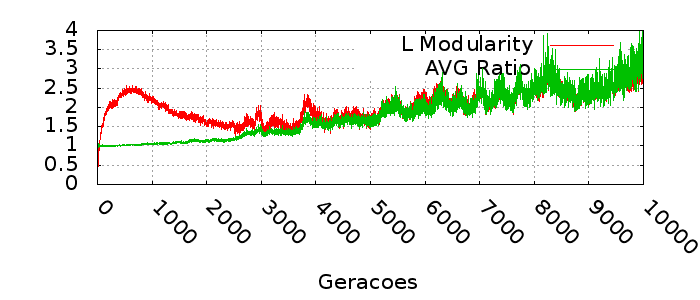
\includegraphics[width=70mm, height=30mm]{figuras/IntSelStats60.png}}\\
      \vspace{-18pt}
      \subfloat [$\Delta_S = 0.07$]{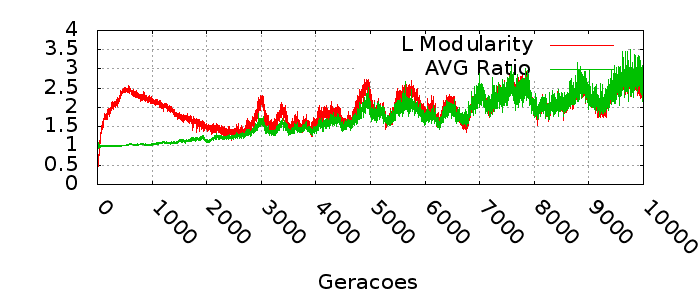
\includegraphics[width=70mm, height=30mm]{figuras/IntSelStats70.png}}\vspace{11pt}
      \subfloat [$\Delta_S = 0.08$]{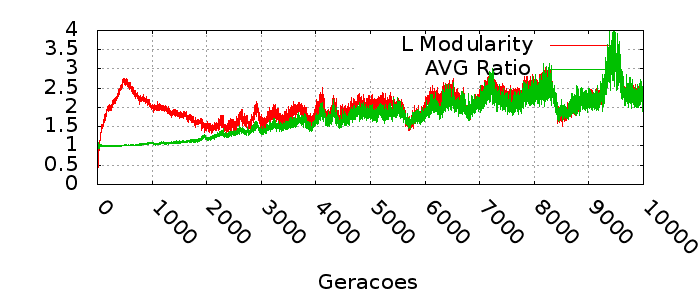
\includegraphics[width=70mm, height=30mm]{figuras/IntSelStats80.png}}\\
      \vspace{-18pt}
      \subfloat [$\Delta_S = 0.09$]{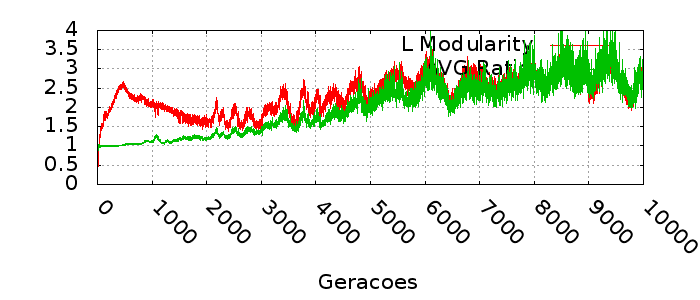
\includegraphics[width=70mm, height=30mm]{figuras/IntSelStats90.png}}\vspace{11pt}
      \subfloat [$\Delta_S = 0.1$]{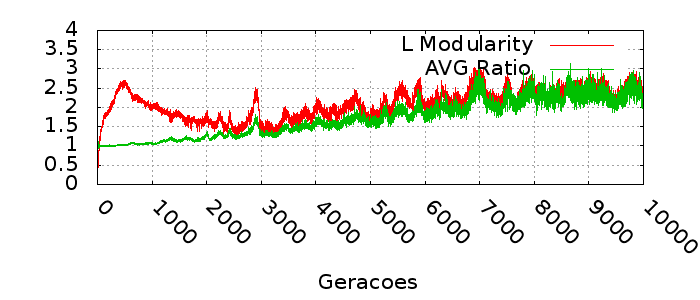
\includegraphics[width=70mm, height=30mm]{figuras/IntSelStats100.png}}\\
      \caption{ AVG-Ratio e modularidade $L$ para corridas com
         $\mu/\mu_B = 5$, $Ne = 2.500$, $m/p=2$, sofrendo seleção
         estabilizadora correlacionada com 2 módulos e seleção direcional com
         diferentes valores de $\Delta_S$.}
      \label{IntSelStats10100}
   \end{figure}



\begin{figure}[htbp]
  \centering
  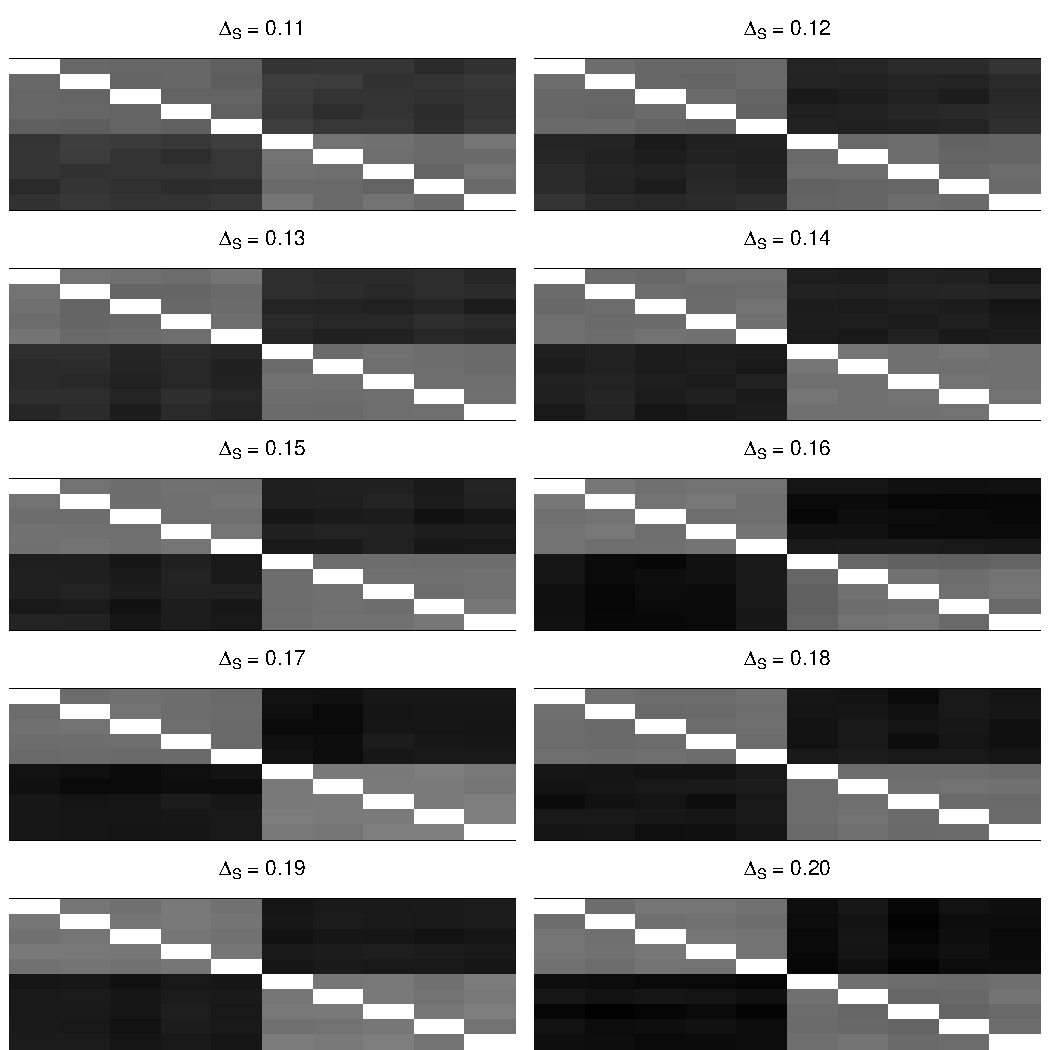
\includegraphics[width=150mm, height=180mm]{figuras/MatBDirecionalIntSel1120}
   \caption{Matriz final média de 10 corridas com
   $\mu/\mu_B = 5$, $Ne = 1.000$, $m/p=2$, sofrendo seleção estabilizadora correlacionada com 2
   módulos e seleção direcional com diferentes valores de $\Delta_S$.}
  \label{MatBIntSel1120}
\end{figure}



   \begin{figure}[htbp]
      \centering
      \subfloat [$\Delta_S = 0.11$]{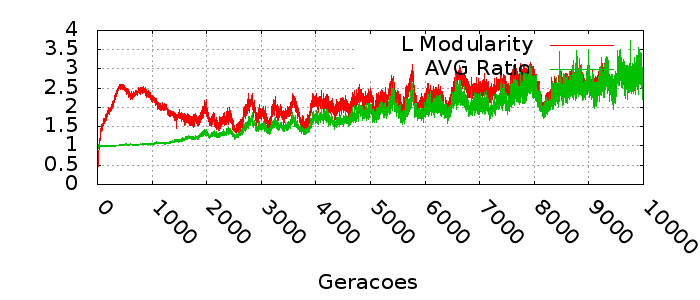
\includegraphics[width=70mm, height=30mm]{figuras/IntSelStats110.png}}\vspace{11pt}
      \subfloat [$\Delta_S = 0.12$]{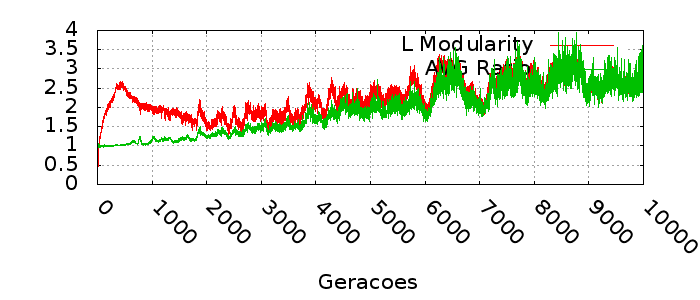
\includegraphics[width=70mm, height=30mm]{figuras/IntSelStats120.png}}\\ 
      \vspace{-18pt}
      \subfloat [$\Delta_S = 0.13$]{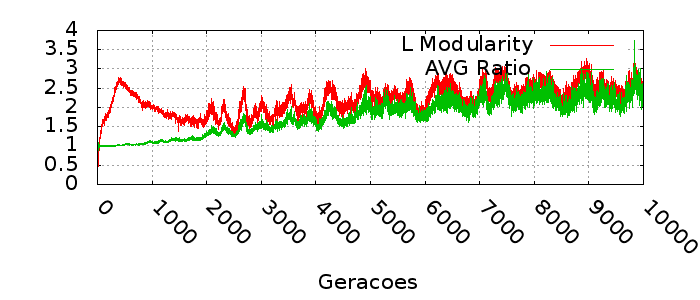
\includegraphics[width=70mm, height=30mm]{figuras/IntSelStats130.png}}\vspace{11pt} 
      \subfloat [$\Delta_S = 0.14$]{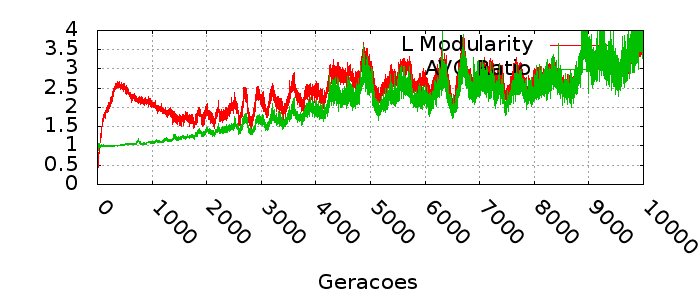
\includegraphics[width=70mm, height=30mm]{figuras/IntSelStats140.png}}\\
      \vspace{-18pt}
      \subfloat [$\Delta_S = 0.15$]{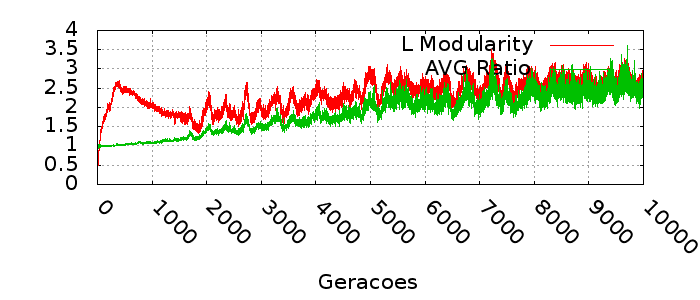
\includegraphics[width=70mm, height=30mm]{figuras/IntSelStats150.png}}\vspace{11pt}
      \subfloat [$\Delta_S = 0.16$]{\includegraphics[width=70mm, height=30mm]{figuras/IntSelStats160.png}}\\
      \vspace{-18pt}
      \subfloat [$\Delta_S = 0.17$]{\includegraphics[width=70mm, height=30mm]{figuras/IntSelStats170.png}}\vspace{11pt}
      \subfloat [$\Delta_S = 0.18$]{\includegraphics[width=70mm, height=30mm]{figuras/IntSelStats180.png}}\\
      \vspace{-18pt}
      \subfloat [$\Delta_S = 0.19$]{\includegraphics[width=70mm, height=30mm]{figuras/IntSelStats190.png}}\vspace{11pt}
      \subfloat [$\Delta_S = 0.2$]{\includegraphics[width=70mm, height=30mm]{figuras/IntSelStats200.png}}\\
      \caption{ AVG-Ratio e modularidade $L$ para corridas com
         $\mu/\mu_B = 5$, $Ne = 2.500$, $m/p=2$, sofrendo seleção
         estabilizadora correlacionada com 2 módulos e seleção direcional com
         diferentes valores de $\Delta_S$.}
      \label{IntSelStats110200}
   \end{figure}


Outra questão relevante é o quão estáveis são os padrões de covariação
modulares gerados pela seleção direcional e estabilizadora. 
Para responder a essa pergunta nós sujeitamos populações de tamanhos
diferentes a uma mesma pressão seletiva intensa durante 5.000 gerações
(período suficiente para o surgimento de módulos), seguidas de 5.000
gerações de seleção estabilizadora correlacionada. 
Apesar da diferença entre as correlações dentro e entre módulos
diminuir, ainda observamos uma distinção estável entre elas (figura
\ref{posselecao} e \ref{posselecaoStats}). 
O efeito do tamanho populacional é especialmente marcante nessas
condições, com populações grandes se mostrando mais eficientes na
manutenção prolongada dos padrões estabelecidos pela seleção direcional
(figuras \ref{posselecao} e \ref{posselecaoStats}). 


\begin{figure}[htbp]
  \centering
  \subfloat [$Ne = 250$]{\includegraphics[width=70mm, height=50mm]{figuras/posselecao250.png}}\vspace{11pt}
  \subfloat [$Ne = 500$]{\includegraphics[width=70mm, height=50mm]{figuras/posselecao500.png}}\\
  \vspace{-18pt}
  \subfloat [$Ne = 1.000$]{\includegraphics[width=70mm, height=50mm]{figuras/posselecao1000.png}}\vspace{11pt}
  \subfloat [$Ne = 2.500$]{\includegraphics[width=70mm, height=50mm]{figuras/posselecao2500.png}}\\
  \vspace{-18pt}
  \subfloat [$Ne = 5.000$]{\includegraphics[width=70mm, height=50mm]{figuras/posselecao5000.png}}\vspace{11pt}
  \subfloat [$Ne = 10.000$]{\includegraphics[width=70mm, height=50mm]{figuras/posselecao10000.png}}\\
  \caption{Evolução da correlação entre dez caracteres ligados por efeitos
  pleiotrópicos controlados por uma matriz $B$ variável, sofrendo seleção estabilizadora correlacionada e seleção
  direcional para mudança correlacionada dentro dos módulos
  durante as 5.000 primeiras gerações, seguidos de 5.000 gerações de
  seleção estabilizadora correlacionada ($\Delta_S = 0.2$, $\mu/\mu_B=5$, $m/p=2$).}
  \label{posselecao}
\end{figure}



\begin{figure}[htbp]
  \centering
  \subfloat [$Ne = 250$]{\includegraphics[width=70mm, height=50mm]{figuras/PosSelStatsNe250.png}}\vspace{11pt}
  \subfloat [$Ne = 500$]{\includegraphics[width=70mm, height=50mm]{figuras/PosSelStatsNe500.png}}\\
  \vspace{-18pt}
  \subfloat [$Ne = 1.000$]{\includegraphics[width=70mm, height=50mm]{figuras/PosSelStatsNe1000.png}}\vspace{11pt}
  \subfloat [$Ne = 2.500$]{\includegraphics[width=70mm, height=50mm]{figuras/PosSelStatsNe2500.png}}\\
  \vspace{-18pt}
  \subfloat [$Ne = 5.000$]{\includegraphics[width=70mm, height=50mm]{figuras/PosSelStatsNe5000.png}}\vspace{11pt}
  \subfloat [$Ne = 10.000$]{\includegraphics[width=70mm, height=50mm]{figuras/PosSelStatsNe10000.png}}\\
  \caption{Evolução de modularidade $L$ e AVG-Ratio para as correlações
     apresentadas na figura \ref{posselecao} ($\Delta_S = 0.2$, $\mu/\mu_B=5$, $m/p=2$).}
  \label{posselecaoStats}
\end{figure}



\begin{figure}[htbp]
  \centering
  \subfloat [$Ne = 250$]{\includegraphics[width=70mm, height=50mm]{figuras/posselecaoSemEstab250.png}}\vspace{11pt}
  \subfloat [$Ne = 500$]{\includegraphics[width=70mm, height=50mm]{figuras/posselecaoSemEstab500.png}}\\
  \vspace{-18pt}
  \subfloat [$Ne = 1.000$]{\includegraphics[width=70mm, height=50mm]{figuras/posselecaoSemEstab1000.png}}\vspace{11pt}
  \subfloat [$Ne = 2.500$]{\includegraphics[width=70mm, height=50mm]{figuras/posselecaoSemEstab2500.png}}\\
  \vspace{-18pt}
  \subfloat [$Ne = 5.000$]{\includegraphics[width=70mm, height=50mm]{figuras/posselecaoSemEstab5000.png}}\vspace{11pt}
  \subfloat [$Ne = 10.000$]{\includegraphics[width=70mm, height=50mm]{figuras/posselecaoSemEstab10000.png}}\\
  \caption{Evolução da correlação entre dez caracteres ligados por efeitos
  pleiotrópicos controlados por uma matriz $B$ variável, sofrendo
  seleção estabilizadora correlacionada e seleção direcional para
  mudança correlacionada dentro dos módulos durante as 5.000
  primeiras gerações, seguidos de 5.000 gerações de seleção
  estabilizadora não correlacionada ($\Delta_S = 0.2$, $\mu/\mu_B=5$,
  $m/p=2$).}
  \label{posselecaoSemEstab}
\end{figure}



\begin{figure}[htbp]
  \centering
  \subfloat [$Ne = 250$]{\includegraphics[width=70mm, height=50mm]{figuras/SemEstabPosSelStatsNe250.png}}\vspace{11pt}
  \subfloat [$Ne = 500$]{\includegraphics[width=70mm, height=50mm]{figuras/SemEstabPosSelStatsNe500.png}}\\
  \vspace{-18pt}
  \subfloat [$Ne = 1.000$]{\includegraphics[width=70mm, height=50mm]{figuras/SemEstabPosSelStatsNe1000.png}}\vspace{11pt}
  \subfloat [$Ne = 2.500$]{\includegraphics[width=70mm, height=50mm]{figuras/SemEstabPosSelStatsNe2500.png}}\\
  \vspace{-18pt}
  \subfloat [$Ne = 5.000$]{\includegraphics[width=70mm, height=50mm]{figuras/SemEstabPosSelStatsNe5000.png}}\vspace{11pt}
  \subfloat [$Ne = 10.000$]{\includegraphics[width=70mm, height=50mm]{figuras/SemEstabPosSelStatsNe10000.png}}\\
  \caption{Evolução de modularidade $L$ e AVG-Ratio para as correlações
     apresentadas na figura \ref{posselecao} ($\Delta_S = 0.2$, $\mu/\mu_B=5$, $m/p=2$).}
  \label{posselecaoSemEstabStats}
\end{figure}


Ainda na questão da estabilidade dos padrões de covariação, o papel da
seleção estabilizadora correlacionada pode ser avaliado sujeitando as
populações à seleção direcional e estabilizadora correlacionada por 5.000
gerações, seguidas de 5.000 gerações de seleção estabilizadora não
correlacionada, apenas mantendo a média de cada caráter individualmente.
Nas figura \ref{posselecaoSemEstab} e \ref{posselecaoSemEstabStats}
podemos ver a importância da seleção estabilizadora correlacionada na
manutenção dos padrões modulares gerados pela seleção direcional. 
Comparando cada tamanho populacional mostrado nas figuras
\ref{posselecao}, \ref{posselecaoStats} e \ref{posselecaoSemEstab},
\ref{posselecaoSemEstabStats} podemos ver uma degradação muito mais
acentuada dos padrões modulares na ausência da seleção
estabilizadora correlacionada. 

A importância da seleção estabilizadora para explicar padrões de estase
no registro fóssil foi amplamente discutida em \cite{Charlesworth1982a}.
No contexto de padrões de covariação, seleção estabilizadora
correlacionada também foi apontada como uma provável explicação para a
estabilidade de padrões de covariação observados na natureza
\citep{Cheverud1984, Marroig2001, Porto2009}. 
Nossos resultados dão credibilidade a essa hipótese. 
A origem dessa seleção estabilizadora pode ser atribuída a fatores
internos dos organismos, como restrições ontogenéticas responsáveis pela
coesão entre as partes do indivíduo. 
Como essas restrições estão sempre presentes, a seleção correlacionada
está sempre presente e os padrões tendem a se manter estáveis. 

Um parâmetro ainda não mencionado é o número de alelos $m$ envolvidos na
determinação do valor fenotípico de cada um dos $p$ caracteres. 
No nosso esquema de simulação, aumentar o valor da razão $m/p$ é análogo
a aumentar a força de recombinação, pois o valor de $m$ define o número
de unidades recombinantes segregando na população. 
Podemos pensar em $m$ como o número de cromossomos no genoma do
indivíduo, em vez de pensar nele como número de alelos individualmente. 
Até agora a razão $m/p$ foi mantida em 2, um valor suficiente para
promover respostas complexas de todos os caracteres mas ainda
computacionalmente viável. 
Razões maiores de $m/p$ teoricamente aumentam o espaço de variação
possível para população, pois mais genes estão disponíveis para atuar
sobre cada caráter, separadamente ou não. 
A figura \ref{MB} mostra como o aumento na razão $m/p$ afeta a evolução
das correlações fenotípicas nas populações sujeitas a seleção direcional
intensa e seleção estabilizadora correlacionada. 
Vemos na figura \ref{MB} que o aumento do número de alelos torna o
sistema mais lento em adquirir um caráter modular. 
Isso pode ser associado com o aumento na recombinação, que age na
direção oposta a das forças seletivas direcionais e estabilizadora
correlacionada. 
Isso nos levou a crer que tempos mais longos de seleção poderiam gerar o
mesmo resultado que o obtido com valores baixos de $m/p$. 
Na figura \ref{MBLR} vemos duas corridas longas, de 20.000 gerações, com
$m/p = 9$ e $10$, mostrando o tempo de estabilização mais longo e a
modularidade mais discreta, com menor diferença nas correlações dentro
de e entre módulos. 
Isso novamente pode ser associado à força de recombinação aumentada. 

Com isso exploramos algumas das combinações de parâmetros possíveis
nesses modelos, além das suas interpretações e consequências na evolução
do padrão de correlação nas populações simuladas. 
Um passo futuro seria estimar os equivalentes desses parâmetros em
populações naturais e simular populações ``equivalentes'' às de
interesse. 
Outro caminho possível é criar diagramas de fase para parâmetros
desconhecidos ou de medição difícil a partir dos parâmetros mensuráveis, 
limitando assim sua faixa plausível e auxiliando a interpretação da
história evolutiva de determinado grupo. 
No próximo capitulo vamos utilizar combinações plausíveis de parâmetros
no nosso modelo para testar a viabilidade de trajetórias evolutivas que
levem a modularidade variacional. 

\begin{figure}[htbp]
   \centering
  \subfloat [$m/p = 2$]{\includegraphics[width=70mm, height=40mm]{figuras/MB20.png}}\vspace{11pt}
  \subfloat [$m/p = 3$]{\includegraphics[width=70mm, height=40mm]{figuras/MB30.png}}\\
  \vspace{-18pt}
  \subfloat [$m/p = 4$]{\includegraphics[width=70mm, height=40mm]{figuras/MB40.png}}\vspace{11pt}
  \subfloat [$m/p = 5$]{\includegraphics[width=70mm, height=40mm]{figuras/MB50.png}}\\
  \vspace{-18pt}
  \subfloat [$m/p = 6$]{\includegraphics[width=70mm, height=40mm]{figuras/MB60.png}}\vspace{11pt}
  \subfloat [$m/p = 7$]{\includegraphics[width=70mm, height=40mm]{figuras/MB70.png}}\\
  \vspace{-18pt}
  \subfloat [$m/p = 8$]{\includegraphics[width=70mm, height=40mm]{figuras/MB80.png}}\vspace{11pt}
  \subfloat [$m/p = 9$]{\includegraphics[width=70mm, height=40mm]{figuras/MB90.png}}\\
  \caption{Evolução da correlação entre dez caracteres ligados por efeitos
  pleiotrópicos controlados por uma função ontogenética linear binária
  variável sofrendo seleção estabilizadora correlacionada e seleção
  direcional intensa para mudança correlacionada dentro dos módulos,
  para diferentes valores do número de alelos. ($Ne=5.000$, $\mu/\mu_B=5$, $\Delta_S=0.2$)}
  \label{MB}
\end{figure}
\begin{figure}[htbp]
  \centering
  \subfloat [$m/p = 9$]{\includegraphics[width=150mm, height=80mm]{figuras/MBLR90.png}}\vspace{11pt}
  \vspace{-18pt}
  \subfloat [$m/p = 10$]{\includegraphics[width=150mm, height=80mm]{figuras/MBLR100.png}}\vspace{11pt}
  \caption{Evolução da correlação entre dez caracteres ligados por efeitos
  pleiotrópicos controlados por uma função ontogenética linear binária
  variável sofrendo seleção estabilizadora correlacionada e seleção
  direcional intensa para mudança correlacionada dentro dos módulos,
  para diferentes valores do número de alelos. ($Ne=5.000$, $\mu/\mu_B=5$, $\Delta_S=0.2$)}
  \label{MBLR}
\end{figure}
	% Capítulo 3: ...
\pagestyle{empty}
\cleardoublepage
\pagestyle{fancy}
\chapter{Considerações Finais}
\label{cap5}

Neste trabalho procuramos trazer uma abordagem matemática/computacional
tipicamente utilizada em sistemas físicos para o estudo de
modularidade. 
O simples ato de tentar reproduzir o comportamento de um sistema natural
complexo através de interações simples das suas partes nos leva a um melhor
entendimento desse sistema, no sentido de evidenciar quais os
ingredientes necessários para que o sistema se comporte de determinada
maneira, mesmo que esses ingredientes sejam difíceis de ser medidos ou
observados na natureza. 
Além disso, os parâmetros utilizados na criação do modelo tem
interpretações no mundo natural. 
O sistema computacional permite com que estudemos as consequências da
variação desses parâmetros em diversas situações inacessíveis ao
experimento ou à medição retrospectiva. 
Podemos também restringir o espaço de variação desses parâmetros,
facilitando sua estimativa por vias indiretas ou limitando sua
influência em outros processos de interesse. 

Nosso trabalho também se coloca como a primeira tentativa de simulação
de sistemas morfológicos complexos o suficiente para permitir o
surgimento de estruturas de modularidade variacional complexas. 
Tentativas anteriores se limitam a apenas simular um, ou um número
pequeno, de traços. 
Por isso também as exigências computacionais são consideravelmente
maiores no nosso caso. 
Assim, nos limitamos a um tratamento basicamente qualitativo do problema
de evolução da modularidade. 
Nesse contexto, mostramos que seleção direcional correlacionada é
necessária para o surgimento de módulos variacionais. 
Além disso, para a manutenção desses módulos precisamos de seleção
estabilizadora correlacionada, mantendo o padrão de variação
estabelecido pela seleção direcional.
Mostramos ainda que a ação conjunta de seleção direcional e
estabilizadora é suficiente para criar padrões covariação complexos, com
varias classes de correlação diferentes surgindo pela interação entre
os dois tipos de seleção.
Com uma implementação mais sofisticada dos
nossos algoritmos, aliada a um poder computacional maior, acreditamos
que uma extensão quantitativa dos resultados seja não só possível como
bastante proveitosa. 

Outra extensão clara é a de utilizar o nosso modelo para reproduzir
padrões específicos de diversificação observados na natureza. 
Por exemplo, um padrão claro em mamíferos é a diferença entre os níveis
de integração total, característica extremamente variável entre os
grupos, apesar do padrão de integração ser relativamente estável
\cite{Porto2009}. 
Quais cenários evolutivos e tipos de seleção e populações podem levar a
extrema diferença de integração observada entre babuínos e grandes
primatas?
A mesma pergunta pode ser feita em relação aos valores altíssimos de
integração presentes em marsupiais. 
Estes são apenas exemplos de problemas em aberto que podem ser abordados
por meio de simulações semelhantes às desenvolvidas neste trabalho. 
Para abordar esses problemas, poderíamos estudar sistemas já com padrões
modulares estabelecidos e simular situações capazes de alterar esses padrões 
nas diferentes populações. 
No momentos nossas populações sempre são inciadas totalmente integradas
ou desintegradas, seria interessante estudar a interação da seleção com
padrões já estabelecidos.
Consequências evolutivas claras, na forma de seleção indireta, são
previstas pela teoria de genética quantitativa quantitativa
\citep{Lande1983, Barton1987}, mas essas situações não foram abordadas
computacionalmente em sistemas de muitos traços.

Ainda existem muitas extensões possíveis ao nosso modelo. 
Eventos populacionais, como gargalos ou episódios consecutivos de
seleção ou mesmo seleção dependente de frequência podem ter
consequências interessantes. 
O estudos de especiação ou diferenciação entre populações filhas, com
diversas filogenias também são possíveis. 
Inclusão de interação entre populações, como migração ou competição por
recursos ou qualquer outro tipo de interação ecológica pode ser incluído
no contexto de simulação de traços quantitativos. 
	% Capítulo 4: Considerações Finais

% Formato da bibliografia
\bibliographystyle{apalike}
% Arquivo .bib
\bibliography{Mestrado}

% Apêndice(s)
\appendix
\chapter{Primeiro apêndice}
Apêndices são opcionais, mas podem ser usados, por exemplo, para incluir tabelas com os dados brutos.


% Fim do texto
\end{document}
